% Plant Physiology Supplemental Data
\documentclass[11pt]{article}
\usepackage[margin=2cm]{geometry}
\usepackage{graphicx}
\usepackage{microtype}
\setlength{\emergencystretch}{3em}
\usepackage{caption}
\usepackage[authoryear,round]{natbib}
\usepackage{amsmath,amssymb}
\usepackage[hidelinks]{hyperref}
\captionsetup{labelformat=empty,font=small}
\begin{document}
\begin{center}
{\Large\textbf{Supplemental Data}}\\[6pt]
The aspartate-to-homoserine pathway recurs across maize grain amino acids, soil nitrogen, and yield selection\\[4pt]
Tandukar, Fitzsimmons, Flint-Garcia, Angelovici, and Rell\'an-\'Alvarez
\end{center}

\section*{Supplemental Methods}

\subsection*{Plant material}

\paragraph*{Goodman--Buckler maize association panel}
The Goodman--Buckler maize association panel \citep{FlintGarcia2005Goodman} was grown at the Genetics Farm near Columbia, Missouri, in 2017 and 2018, with two replicates per year in a randomized complete block design. Of the 282 lines in the panel, 280 were grown successfully. Thirteen kernels of each line were planted in a 10-foot row and self-pollinated. At physiological maturity, ears were harvested and husked, and the ears were dried at 40\,$^{\circ}$C and $<$20\% relative humidity for 5 days. Ears from each line were shelled and bulked within each replicate and year, giving four composite grain samples per line. For amino acid analysis, 25 random kernels from each bulked sample were ground and prepared for extraction and quantification.

\paragraph*{B64 $\times$ CML14 mapping population}
The B64 $\times$ CML14 mapping population was developed by crossing B64 and CML14, the Goodman--Buckler lines with the lowest and highest grain free Asn, respectively. Field design, harvest, and sample preparation for the F$_{2:3}$ families are described in \citet{Fitzsimmons2026KernelKitchen}.
% TODO (check with Sarah): drying is 41 C and 20% relative humidity here but 40 C and <20% for the Goodman-Buckler panel

\paragraph*{Maize landraces}
We used 3,107 georeferenced maize landrace accessions from the CIMMYT International Germplasm Bank \citep{RomeroNavarro2017Landraces}, collected in 28 countries and territories across Mesoamerica (2,296), South America (667), and the Caribbean (144) for which environmental variable such as soil N values were available at the collection sites.

\paragraph*{Indian Chief and Jarvis recurrent-selection populations}
We used two open-pollinated populations, Indian Chief and Jarvis Golden Prolific, from a program of reciprocal recurrent selection for grain yield \citep{MollStuber1971,Moll1994}, sampling the base populations (Cycle 0) and the populations after 14 cycles of selection (Cycle 14). Because parents in each population were selected on the yield of their testcrosses with the other population, allele-frequency changes in the two populations are not fully independent. However, the testcrosses were used only for evaluation, and each new cycle was formed by intermating selected plants within the same population, so no alleles were exchanged between the populations.

For amino acid profiling, Indian Chief and Jarvis Cycle 0 and Cycle 14 plants were grown in 2025 at the Central Crops Research Station (Clayton, NC) under standard field management in a randomized complete block design. Whole cobs with fully developed kernels were harvested and stored until analysis.

\subsection*{Phenotyping}

\paragraph*{Amino acid profiling}
PBAAs were extracted and quantified as described in \cite{Yobi2018PBAA}. This protocol utilizes microscale protein hydrolysis and absolute quantification using multiple reaction monitoring-based liquid chromatography–tandem mass spectrometry detection. During acid hydrolysis, Gln and Asn are converted into Glu and Asp, respectively. Therefore, we denote both Gln and Glu as Glx and Asn and Asp as Asx. During the extraction, Trp and Cys were fully destroyed, and Gly was poorly detected, so these three amino acids were excluded from the dataset. In total, 15 PBAAs were analyzed in the Goodman--Buckler panel, with Asx and Glx each representing two amino acids. In Indian Chief and Jarvis, Gly was also quantified, giving 16 PBAAs. FAAs were extracted and quantified as described in \citet{Gu2007LCMS}. Unlike the protocol above, all 20 proteinogenic amino acids were independently and successfully detected using UPLC-MS/MS.

Amino acid-derived N was estimated by weighting each amino acid by its number of N atoms (4 for Arg, 3 for His, 2 for Asn, Gln, Lys, and Trp, and 1 for the others). Protein-bound Asx and Glx, which combine Asp with Asn and Glu with Gln after hydrolysis, were assigned 1.5 N. For the Goodman--Buckler GWAS trait \textit{Total\_N}, amino acid measurements were converted to amino acid-derived nitrogen values by weighting each amino acid by its nitrogen content. For an amino acid $X$, the nitrogen mass fraction was calculated as

\[
\%N_X =
\left(
\frac{n_{N,X}\times M_N}{M_X}
\right)\times 100
\]

where $M_X$ is the molar mass of amino acid $X$, $M_N$ is the molar mass of nitrogen, and $n_{N,X}$ is the number of nitrogen atoms in amino acid $X$. Amino acid-derived nitrogen for each amino acid was then calculated as

\[
N_X\;(\mu g/mg) =
\left(
\frac{n_{N,X}\times M_N}{M_X}
\right)
\times AA_X\;(\mu g/mg)
\]

and summed across amino acids before BLUP estimation and GWAS.
% TODO: confirm the Total_N weighting. These equations weight by N mass fraction, whereas the pool comparisons (Results, Supplemental Table S5) weight by number of N atoms

\paragraph*{Free and protein-bound amino acid pools}
Free and protein-bound pools were compared in the 279 Goodman--Buckler lines with both measurements \citep{Shrestha2022} using paired Wilcoxon signed-rank tests. Amino acid-derived N was calculated as described above. To compare composition on the same basis, free Asp and Asn and free Glu and Gln were combined to match Asx and Glx, and Gly, Trp, and Cys were excluded from the free-pool total.

\paragraph*{Indian Chief and Jarvis amino acid comparisons}
Technical replicates were averaged within each biological sample (Indian Chief Cycle~0 $n = 5$, Cycle~14 $n = 8$, Jarvis Cycle~0 $n = 3$, Cycle~14 $n = 8$). For each sample we calculated total FAA and PBAA per mg and each amino acid’s fraction within its pool. Amino acid-derived N per mg was calculated as described above, and total amino acid-derived N was the sum of FAA- and PBAA-derived N, estimating N in amino acids (not total grain N). Cycle~0 and Cycle~14 were compared within each population with two-sided Wilcoxon rank-sum tests (normal approximation), with Cliff’s $\delta$ as the effect size. $P$ values were Benjamini--Hochberg adjusted within each of four test families, the eight FAA metrics (Supplemental Table~S14), the amino acids within each pool (Supplemental Table~S15), the PBAA metrics (Supplemental Table~S16), and the three amino acid-derived N measures (Supplemental Table~S17). With three Cycle~0 Jarvis samples, the minimum possible $P$ was 0.019.

\paragraph*{Soil nitrogen}
The environmental phenotype, soil total N, was taken from SoilGrids 2.0 \citep{Poggio2021SoilGrids} at 250 m resolution. Values for the 0--5~cm and 5--15~cm layers were assigned to the collection coordinates of each landrace accession, and 0--5 cm was used as the primary GWAS phenotype and 5--15~cm as a check.

\subsection*{Genotyping}

\paragraph*{Goodman--Buckler panel}
The Goodman--Buckler panel was genotyped with the maize HapMap 3.2.1 SNPs for the 282-line panel \citep{Bukowski2018HapMap3}, 4,177,796 SNPs positioned on the B73 AGPv4 assembly. Positions were lifted to B73 RefGen\_v5 (Zm-B73-REFERENCE-NAM-5.0), referred to below as reference genome version 5 (RefGen\_v5), as described under Amino acid GWAS.

\paragraph*{B64 $\times$ CML14 mapping population}
F$_2$ plants were genotyped with the mid-density temperate corn panel of Agriplex Genomics (Cleveland, OH) as described in \citet{Fitzsimmons2026KernelKitchen}.

\paragraph*{Maize landraces}
The landraces were genotyped by genotyping-by-sequencing at about 2$\times$ coverage, with SNP calling and imputation by \citet{RomeroNavarro2017Landraces}. We used 495,755 SNPs positioned on reference genome version 5 for the 3,107 accessions with soil N values.

\paragraph*{Indian Chief and Jarvis}

Each population--cycle group included 96 individuals (384 in total). Paired-end Illumina libraries were prepared with Twist Bioscience kits and sequenced as 2~$\times$~150~bp reads on a NovaSeq 6000, and reads were demultiplexed with \texttt{fqtk} v0.3.1.
% TODO: confirm the exact Twist kit name, and add the tissue sampled and the DNA extraction method

Reads were trimmed/filtered with \texttt{fastp} v0.23.4, QC-checked with \texttt{FastQC} v0.12.1, aligned to RefGen\_v5 (GCF\_902167145.1) using \texttt{BWA-MEM} v0.7.18, and deduplicated with \texttt{Picard MarkDuplicates} v3.1.1. Variants were jointly called with GATK v4.5.0.0 Best Practices (\texttt{CombineGVCFs}, \texttt{GenotypeGVCFs}) and hard-filtered, yielding 52,543,238 SNPs. After removing five low-quality samples, 379 individuals remained. For population structure, we kept biallelic SNPs on the 10 chromosomes with QUAL $\ge 30$, MAF $\ge 0.01$, site depth 221--413, and data in $\ge$50\% of individuals (\texttt{bcftools} v1.18), leaving 512,667 SNPs. Mean depth at these SNPs was 0.73$\times$ per individual (0.32--1.91$\times$); genome-wide coverage including zero-read sites was 0.28--0.38$\times$ per group (\texttt{Picard CollectWgsMetrics}), consistent with low-pass skim sequencing.

\subsection*{Heritability and consistency across years}
Broad-sense heritability ($H^2$) on a line mean basis was estimated on the log scale from the plot records (two years $\times$ two blocks) with the linear mixed model $y \sim 1 + (1|\mathrm{taxa}) + (1|\mathrm{year}) + (1|\mathrm{taxa{:}year}) + (1|\mathrm{year{:}block})$ for 40 free and 76 protein-bound amino acid traits, and the Cullis generalized $H^2$ was computed from the same model. Genomic heritability ($h^2$) was estimated with a VanRaden genomic relationship matrix for the 272 genotyped lines, with 95\% profile-likelihood intervals. Each trait was also fitted with a permuted phenotype, and traits for which the permuted phenotype returned a non-zero $h^2$ were excluded from comparisons of $h^2$ with $H^2$. Consistency across years was measured as the Spearman correlation between 2017 and 2018 line means for the 251 lines grown in both years. For soil N in the landrace panel, genomic heritability was estimated for the 3,107 accessions before and after removing 10 and 50 genotype principal components from the phenotype, and compared with 1,000 permuted phenotypes.

\subsection*{Genome-wide association studies}

\paragraph*{Amino acid GWAS}
We performed GWAS for 78 amino acid phenotypes (Supplemental Table~S2) using phenotype BLUPs and 4,177,796 HapMap 3.2.1 SNPs in the HAPPI pipeline \citep{Slaten2020HAPPI}, applying GAPIT MLM, MLMM, BLINK, and FarmCPU. Significance was set at 5\% Benjamini--Hochberg FDR, calculated separately for each phenotype and model. Because MLMM yielded no significant SNPs, we report results from MLM, BLINK, and FarmCPU. SNP coordinates were lifted from RefGen\_v4 to RefGen\_v5 using the B73 chain file, Twenty one of 2,461 significant SNPs in alignment gaps were moved to the nearest aligned base. Candidate genes were RefGen\_v5 genes within 25 kb of significant SNPs.
% TODO (ask Sarah): state the principal components and kinship used as covariates in the amino acid GWAS

\paragraph*{Soil N GWAS and environmental specificity tests}
GWAS of soil N used the 3,107 landrace accessions and 495,755 SNPs, with MLM, BLINK, and FarmCPU \citep{Slaten2020HAPPI} and three genotype principal components as covariates. Significance was declared at a 5\% Benjamini--Hochberg FDR computed over the full scan for each model, and candidate genes were RefGen\_v5 genes within 25 kb of a significant SNP.

To assess whether soil-N associations reflected geography or climate, we repeated the GWAS for latitude, longitude, elevation \citep{RomeroNavarro2017Landraces}, soil pH, and CEC (0--5 cm) \citep{Poggio2021SoilGrids}, and aridity \citep{Zomer2022Aridity}. For each variable pair, we tested overlap of significant SNPs against chance ($n_1 n_2 / M$, $M = 495{,}755$) with one-sided hypergeometric tests. Independently, we ranked all SNPs by $|r|$ between allele dosage and each site variable across 3,107 accessions. A soil N SNP was classified as environment linked if it was in the top 1\% for any non-N variable, not linked if it was in the top 5\% for soil N but not in the top 1\% for any other variable, and inconclusive otherwise. We compared the fraction of soil N SNPs in the top 1\% for any geographic/environmental variable by binomial tests against the whole genome and against SNPs in the top 1\% for soil N.

For the two focal soil-N SNPs (S1\_16128632, S5\_22338979), we compared soil N among genotypes with Kruskal--Wallis tests ($\varepsilon^2$), followed by Dunn tests with Holm correction, and compared minor-allele carriers vs non-carriers within Mexico and within Central America using Wilcoxon rank-sum tests. These tests do not account for population structure.

\subsection*{QTL mapping}
The genetic map of 610 markers was constructed with R/qtl \citep{Broman2003} as described in \citet{Fitzsimmons2026KernelKitchen}. Best linear unbiased predictions (BLUPs) of free Asp and free Pro were calculated for the 250 F$_{2:3}$ families. QTL scans used Haley--Knott regression, significance thresholds were set at $\alpha = 0.05$ from 1,000 permutations, and support intervals were defined as 1.5-LOD drops from the QTL peak.
% TODO (check with Sarah): the earlier text said that Asp BLUPs were used to construct the genetic map

Genes within the shared 1.5-LOD support interval (chr3:14.37--143.31~Mb) were taken from the reference genome version 5 gene annotation in MaizeGDB \citep{MaizeGDB}, with 192 non-coding genes absent from that annotation added from Ensembl Plants release 62. Genes were annotated with gene name, PANTHER family, protein class, and Gene Ontology terms, and with kernel expression from qTeller \citep{qteller}, which provides RNA-seq transcript abundance across maize kernel tissues and developmental stages (Supplemental Table S8).

\subsection*{Population-genomic analyses of Indian Chief and Jarvis}

\paragraph*{Genotype likelihoods and differentiation between cycles}

Population-genomic statistics were estimated from genotype likelihoods in ANGSD v0.940 \citep{Korneliussen2014ANGSD} for each population–cycle group using identical filters. Per-chromosome site allele-frequency likelihoods (SAF) were computed with the SAMtools genotype-likelihood model from properly paired, unflagged reads (mapping quality $\ge 30$), bases (quality $\ge 20$), and sites with total depth $\ge 2$. The reference genome version 5 allele was set as the major allele, and analyses were restricted to polymorphic sites within each group (SNP likelihood-ratio $P < 10^{-6}$, minor allele frequency $\ge 0.0005$, triallelic sites removed).

Allele-frequency change from Cycle~0 to Cycle~14 was quantified separately in Indian Chief and Jarvis using $F_{ST}$. For each contrast, a joint 2D site-frequency spectrum was estimated from two SAF files with \texttt{winsfs} \citep{Rasmussen2022winsfs} and used as the prior for \texttt{realSFS fst}. Per-site $F_{ST}$ was smoothed along chromosomes with GenWin (spline smoothness 500~kb), which sets window boundaries at spline inflection points \citep{Beissinger2015GenWin}. Each window was summarized by mean per-site $F_{ST}$. Windows at or above the 95th percentile of each population’s window-$F_{ST}$ distribution were retained as candidate regions. These are empirical outliers, not significance thresholds, because drift at these population sizes shifts linked regions together.

To compare candidate regions with different window boundaries, we split the genome at any boundary from either population and assigned each segment the $F_{ST}$ of the Indian Chief and Jarvis windows containing it. Overlap was the number of base pairs in the top 5\% in both populations, assessed against 10,000 circular shifts of the Jarvis track along concatenated chromosomes to preserve window size and clustering. Concordance in window $F_{ST}$ was summarized by Spearman’s correlation across segments.

\paragraph*{Population structure and differentiation between Indian Chief and Jarvis}

Because sequencing depth varied among cycles, we inferred population structure from genotype likelihoods rather than called genotypes. From the filtered VCF, we retained sites with reads in at least half of the 379 individuals and minor allele frequency $\ge 0.05$, then thinned to one site per 10~kb to reduce linkage (82,061 sites). We estimated admixture with NGSadmix \citep{Skotte2013NGSadmix} for $K=2$--5 (three runs per $K$) using the 12,031 sites passing its MAF filter, and chose the largest $K$ for which runs converged. We computed principal components from the genotype-likelihood covariance matrix with PCAngsd \citep{Meisner2018PCAngsd}. We measured differentiation between Indian Chief and Jarvis at Cycle~0 and Cycle~14 using Hudson's $F_{ST}$ \citep{Bhatia2013Fst}, calculated genome-wide and per chromosome from joint site-frequency spectra estimated with \texttt{winsfs} \citep{Rasmussen2022winsfs} from ANGSD SAF files.

\paragraph*{Effective population size}
Because each cycle was formed by intermating the selfed progenies of 20 selected plants within each population \citep{MollStuber1971}, neutral allele-frequency change is expected to follow a Wright--Fisher process with one generation per cycle and an effective population size ($N_e$) of at most 20, the value reached when all selected parents contribute equally.

To compare the observed differentiation with this expectation, we estimated $N_e$ for each population from the allele-frequency change between Cycle~0 and Cycle~14. Per-site allele frequencies were taken from ANGSD \citep{Korneliussen2014ANGSD}, retaining sites with data for at least 30 individuals and the same major and minor alleles in both cycles. Sites were grouped into non-overlapping 250-kb windows (at most 400 randomly chosen sites per window, 8,524 windows in Indian Chief and 8,527 in Jarvis), Hudson's $F_{ST}$ \citep{Bhatia2013Fst} between cycles was computed per window as a ratio of sums, and the genome-wide mean was taken across windows. We then simulated neutral Wright--Fisher drift for 14 generations from the observed Cycle~0 frequencies for $N_e$ = 20, 30, 50, 75, 100, 150, 250, and 500, resampled the simulated frequencies at both time points using the number of individuals with data at each site, and computed $F_{ST}$ with the same estimator. $N_e$ was taken as the value at which the simulated genome-wide mean $F_{ST}$ matched the observed value, interpolating linearly between grid points.

\paragraph*{Candidate window annotation}

Candidate genes were annotated with PANTHER family and protein class \citep{Thomas2022PANTHER} and Gene Ontology terms \citep{GO2026} (Supplemental Tables S20--S21).

\subsection*{Pathway recurrence across analyses}
Pathway membership was obtained from CornCyc (Plant Metabolic Network release 2023, \citealp{Hawkins2021PMN}). For the main test, we used Bonferroni-significant GWAS SNPs $\pm$25~kb ($P < 0.05/4{,}177{,}796$ for amino acids and $P < 0.05/495{,}755$ for soil N) and the top 3\% of windows from each $F_{ST}$ scan. A pathway was considered a hit if any pathway gene overlapped a set interval, and we recorded how many sets hit each pathway. The null distribution was generated from 200,000 permutations by circularly shifting each set's intervals along each chromosome by an independent random offset, preserving interval number, size, spacing, and clustering. For each pathway, $P$ was the fraction of permutations with at least as many set hits as observed (permutation-based empirical $P$). We corrected for testing all 468 pathways with a minimum-$P$ procedure, using one half of the permutations to estimate each pathway's tail probabilities and the other half to obtain the distribution of the smallest $P$ per permutation. To assess sensitivity to thresholds, we repeated the test for 12 combinations of GWAS thresholds (Benjamini--Hochberg FDR 5\%, 3\%, and 1\%, computed per model over the full scan, and Bonferroni) and $F_{ST}$ window thresholds (top 5\%, 3\%, and 1\%), with 20,000 permutations per combination (200,000 for the Bonferroni sets with the top 5\% and 3\% of windows).

\subsection*{Expression of candidate genes under contrasting N supply}
Expression responses of candidate genes to N supply were taken from a reanalysis of published maize RNA-seq studies of root, leaf, shoot, and whole-seedling tissue, listed with their DOIs in Supplemental Table~S22, including six leaf N-deficiency studies \citep{Mu2017LN, Guo2022LN, Ma2021LN, TorresRodriguez2021LN, AlonsoNieves2022LN, Wang2025NRT25}. Reads from each study were quantified against reference genome version 5 with salmon in the nf-core/rnaseq pipeline, and each study was analyzed with DESeq2, testing genes with at least 10 reads in at least two samples. Within each study, contrasts of the same tissue and contrast type were combined by inverse variance, and studies were then pooled with DerSimonian--Laird random-effects meta-analysis. Only replicated contrasts were pooled, and $P$ values were adjusted by the Benjamini--Hochberg method within each tissue and contrast type.
% TODO: cite salmon, nf-core/rnaseq, DESeq2, and DerSimonian & Laird 1986

\clearpage
\section*{Supplemental Figures}
\begin{figure}[p]
\centering
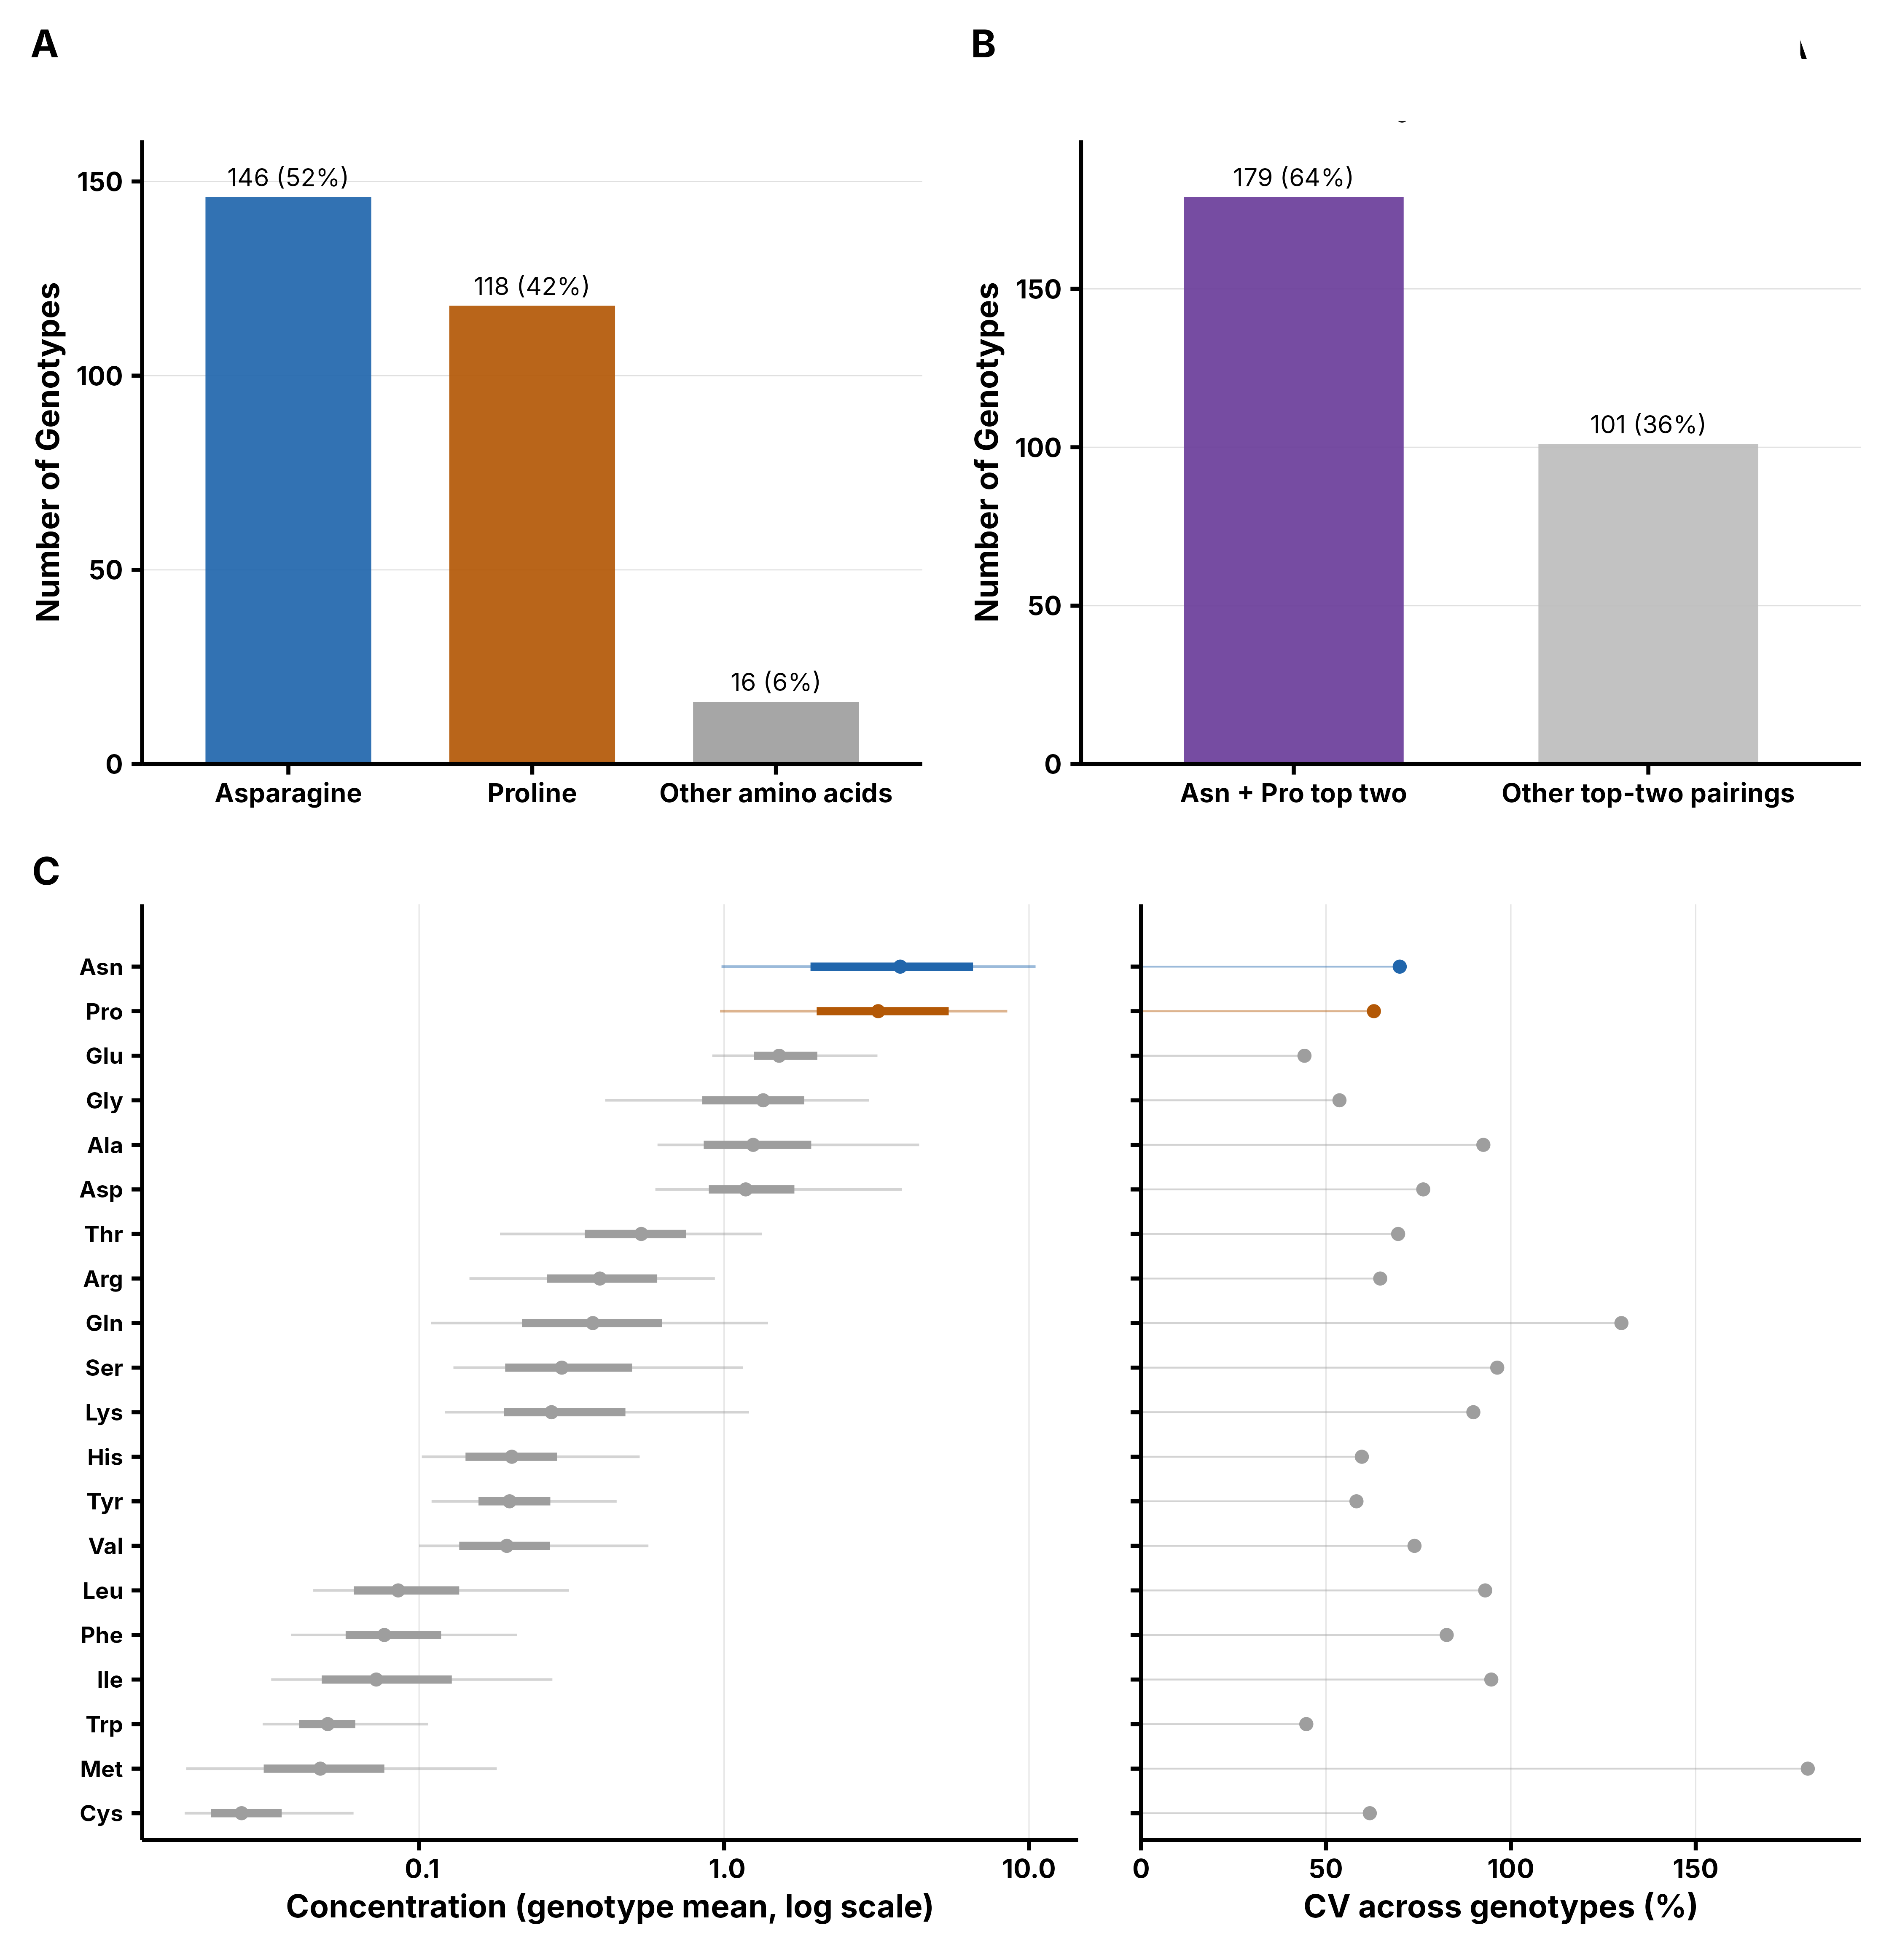
\includegraphics[width=0.95\textwidth]{figures/SuppFig1_FAA_composition.png}
\caption*{\textbf{Supplemental Figure S1.} \textbf{Free amino acid composition of the Goodman--Buckler panel.}
    \textbf{(A)}, Number of genotypes in which each free amino acid ranked most abundant,
    based on genotype means across four replicates ($n = 280$ genotypes).
    \textbf{(B)}, Number of genotypes in which Asn and Pro together occupied the
    top two ranks, in either order.
    \textbf{(C)}, Abundance and variability of each free amino acid. Left, concentration per
    genotype mean on a log scale: point, median across genotypes; thick bar, interquartile
    range; thin bar, 5th--95th percentile; amino acids ordered by median. Right,
    coefficient of variation across genotypes for the same ordering. Asn is shown in blue and Pro in orange throughout.}
\end{figure}
\clearpage

\begin{figure}[p]
\centering
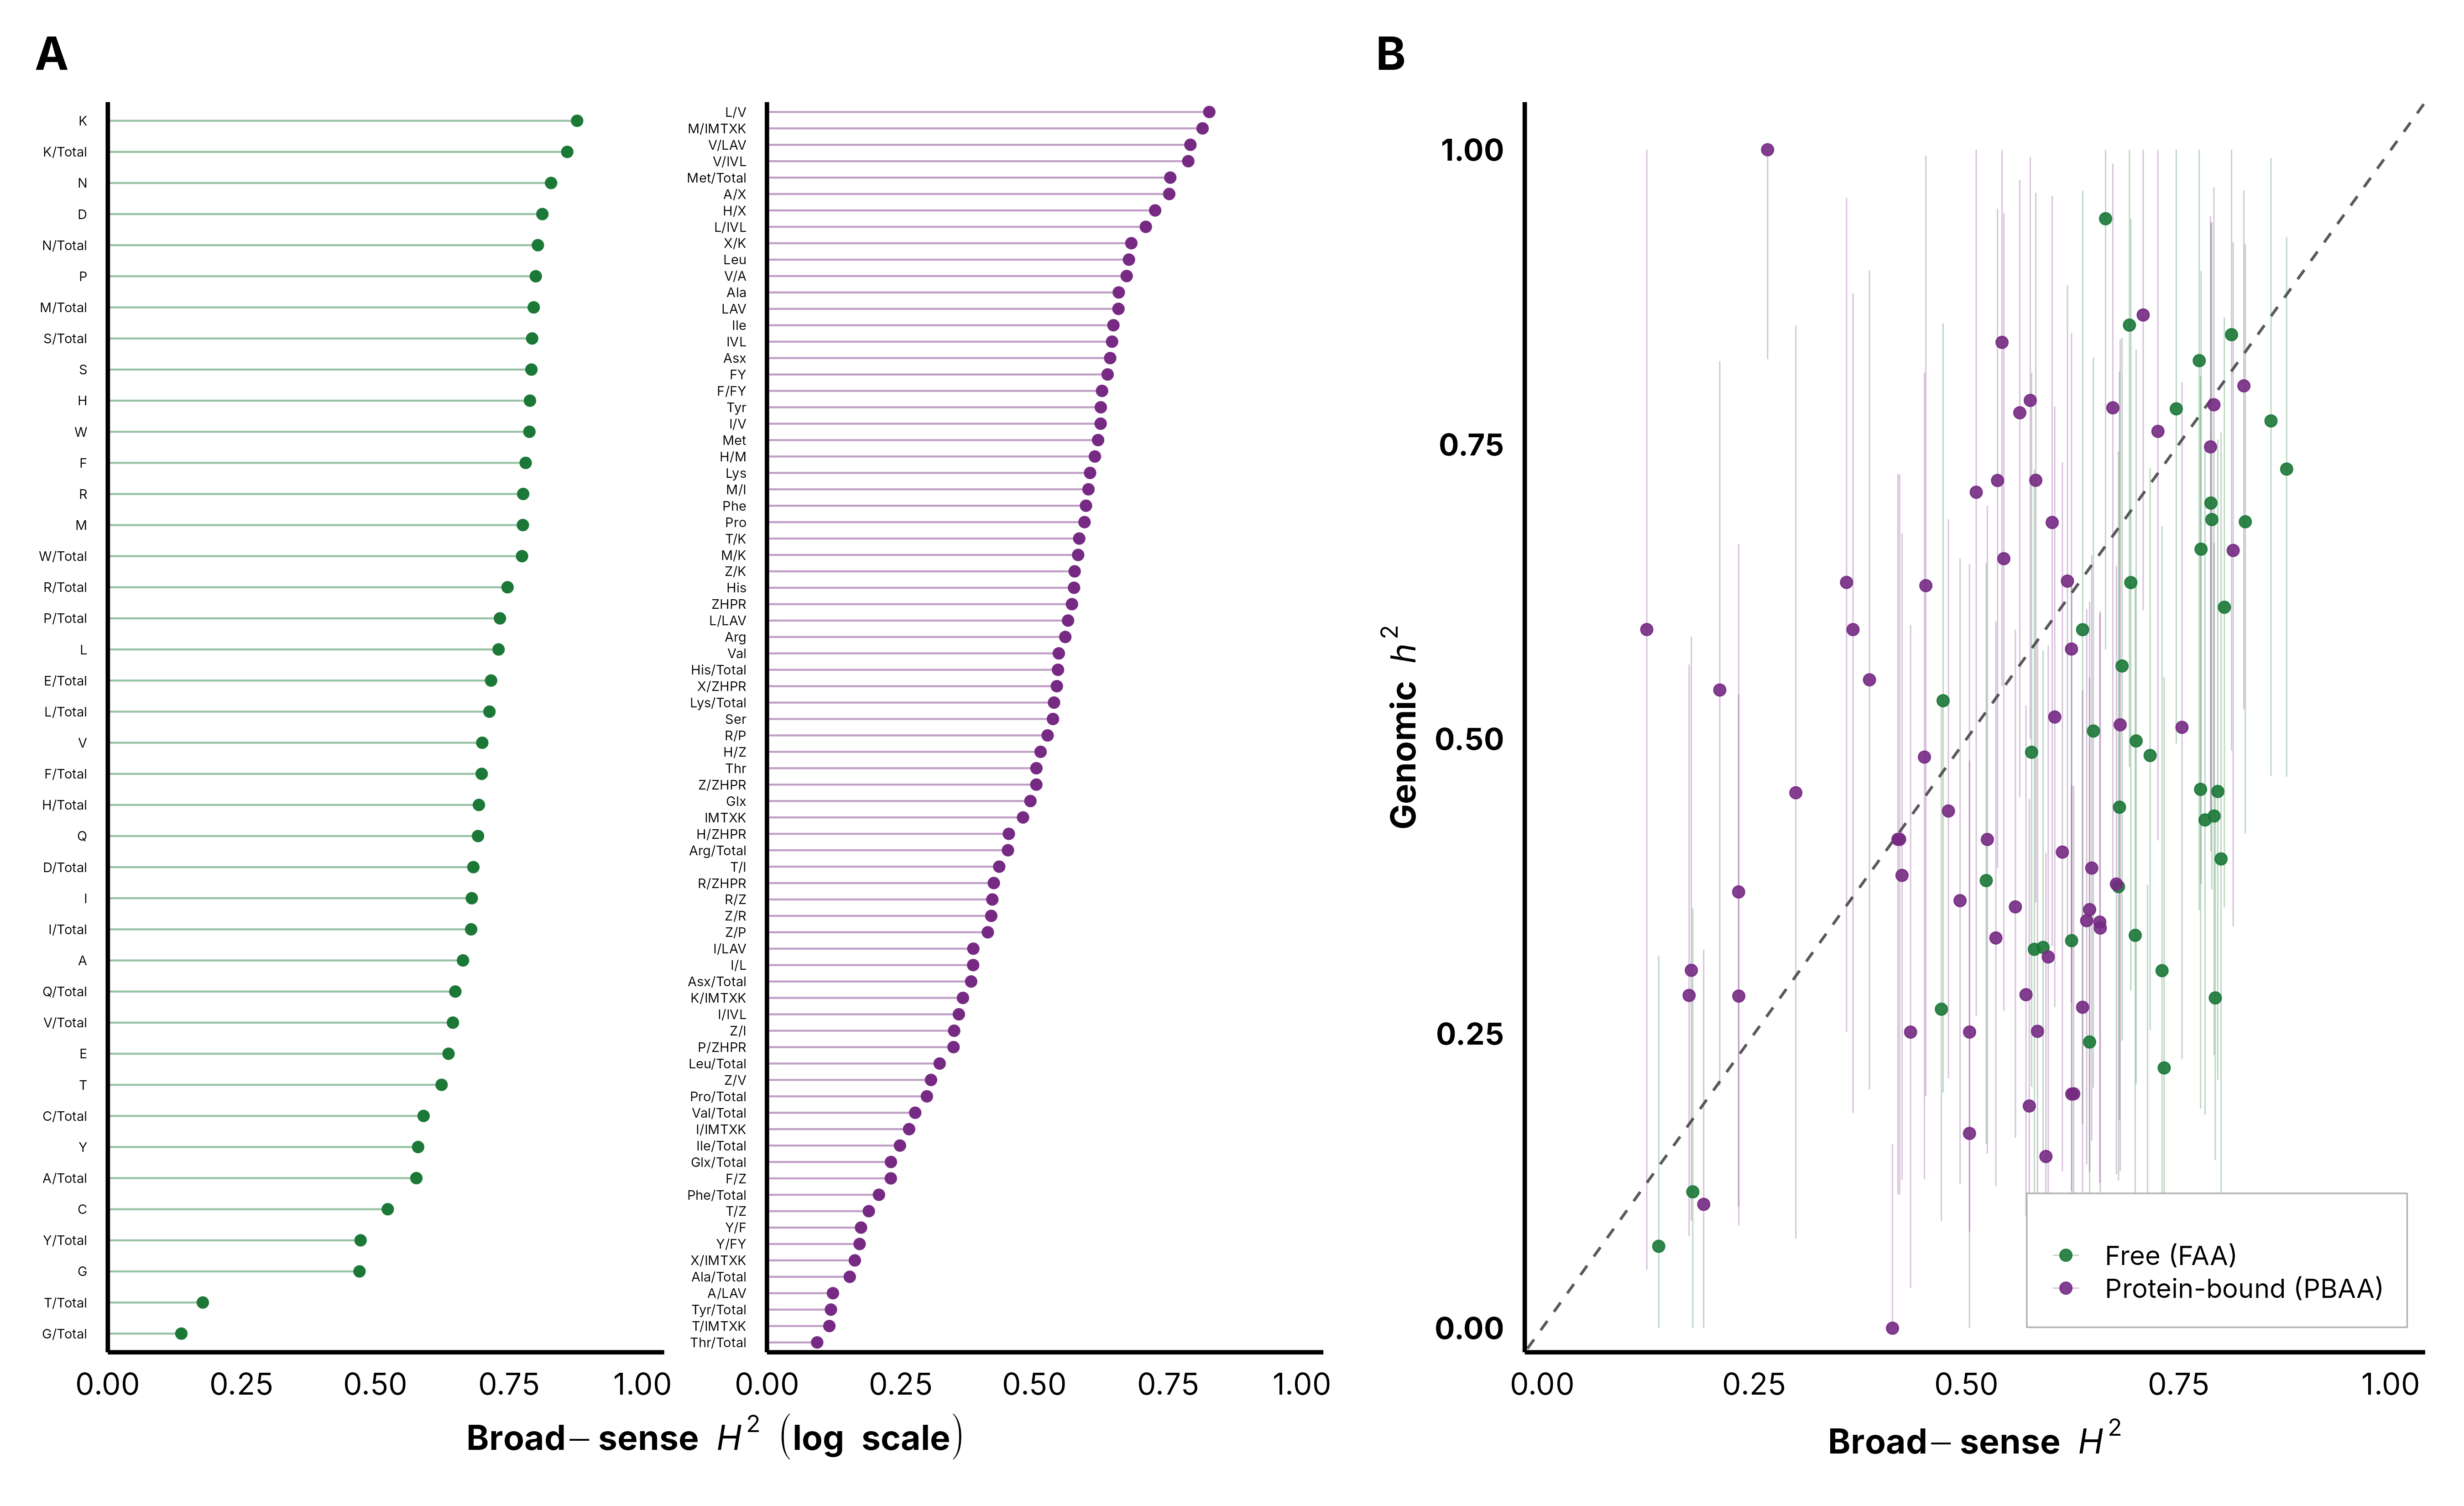
\includegraphics[width=\textwidth]{figures/SuppFig2_heritability.png}
\caption*{\textbf{Supplemental Figure S2.} \textbf{Heritability of grain amino acid phenotypes in the Goodman--Buckler panel.}
    \textbf{(A)}, Broad-sense heritability $H^2$ on a line-mean basis shown for 40 free and 76 protein-bound amino acid traits.
    \textbf{B}, Genomic heritability $h^2$ from a VanRaden genomic relationship matrix plotted against $H^2$, with error bars giving the 95\% profile-likelihood interval on $h^2$ and the dashed line showing $y = x$. Fifteen of
    116 traits returned a non-zero $h^2$ from a permuted phenotype and are excluded from
    panel \textbf{B}; their $H^2$ is unaffected and is retained in panel \textbf{A}.}
\end{figure}
\clearpage

\begin{figure}[p]
\centering
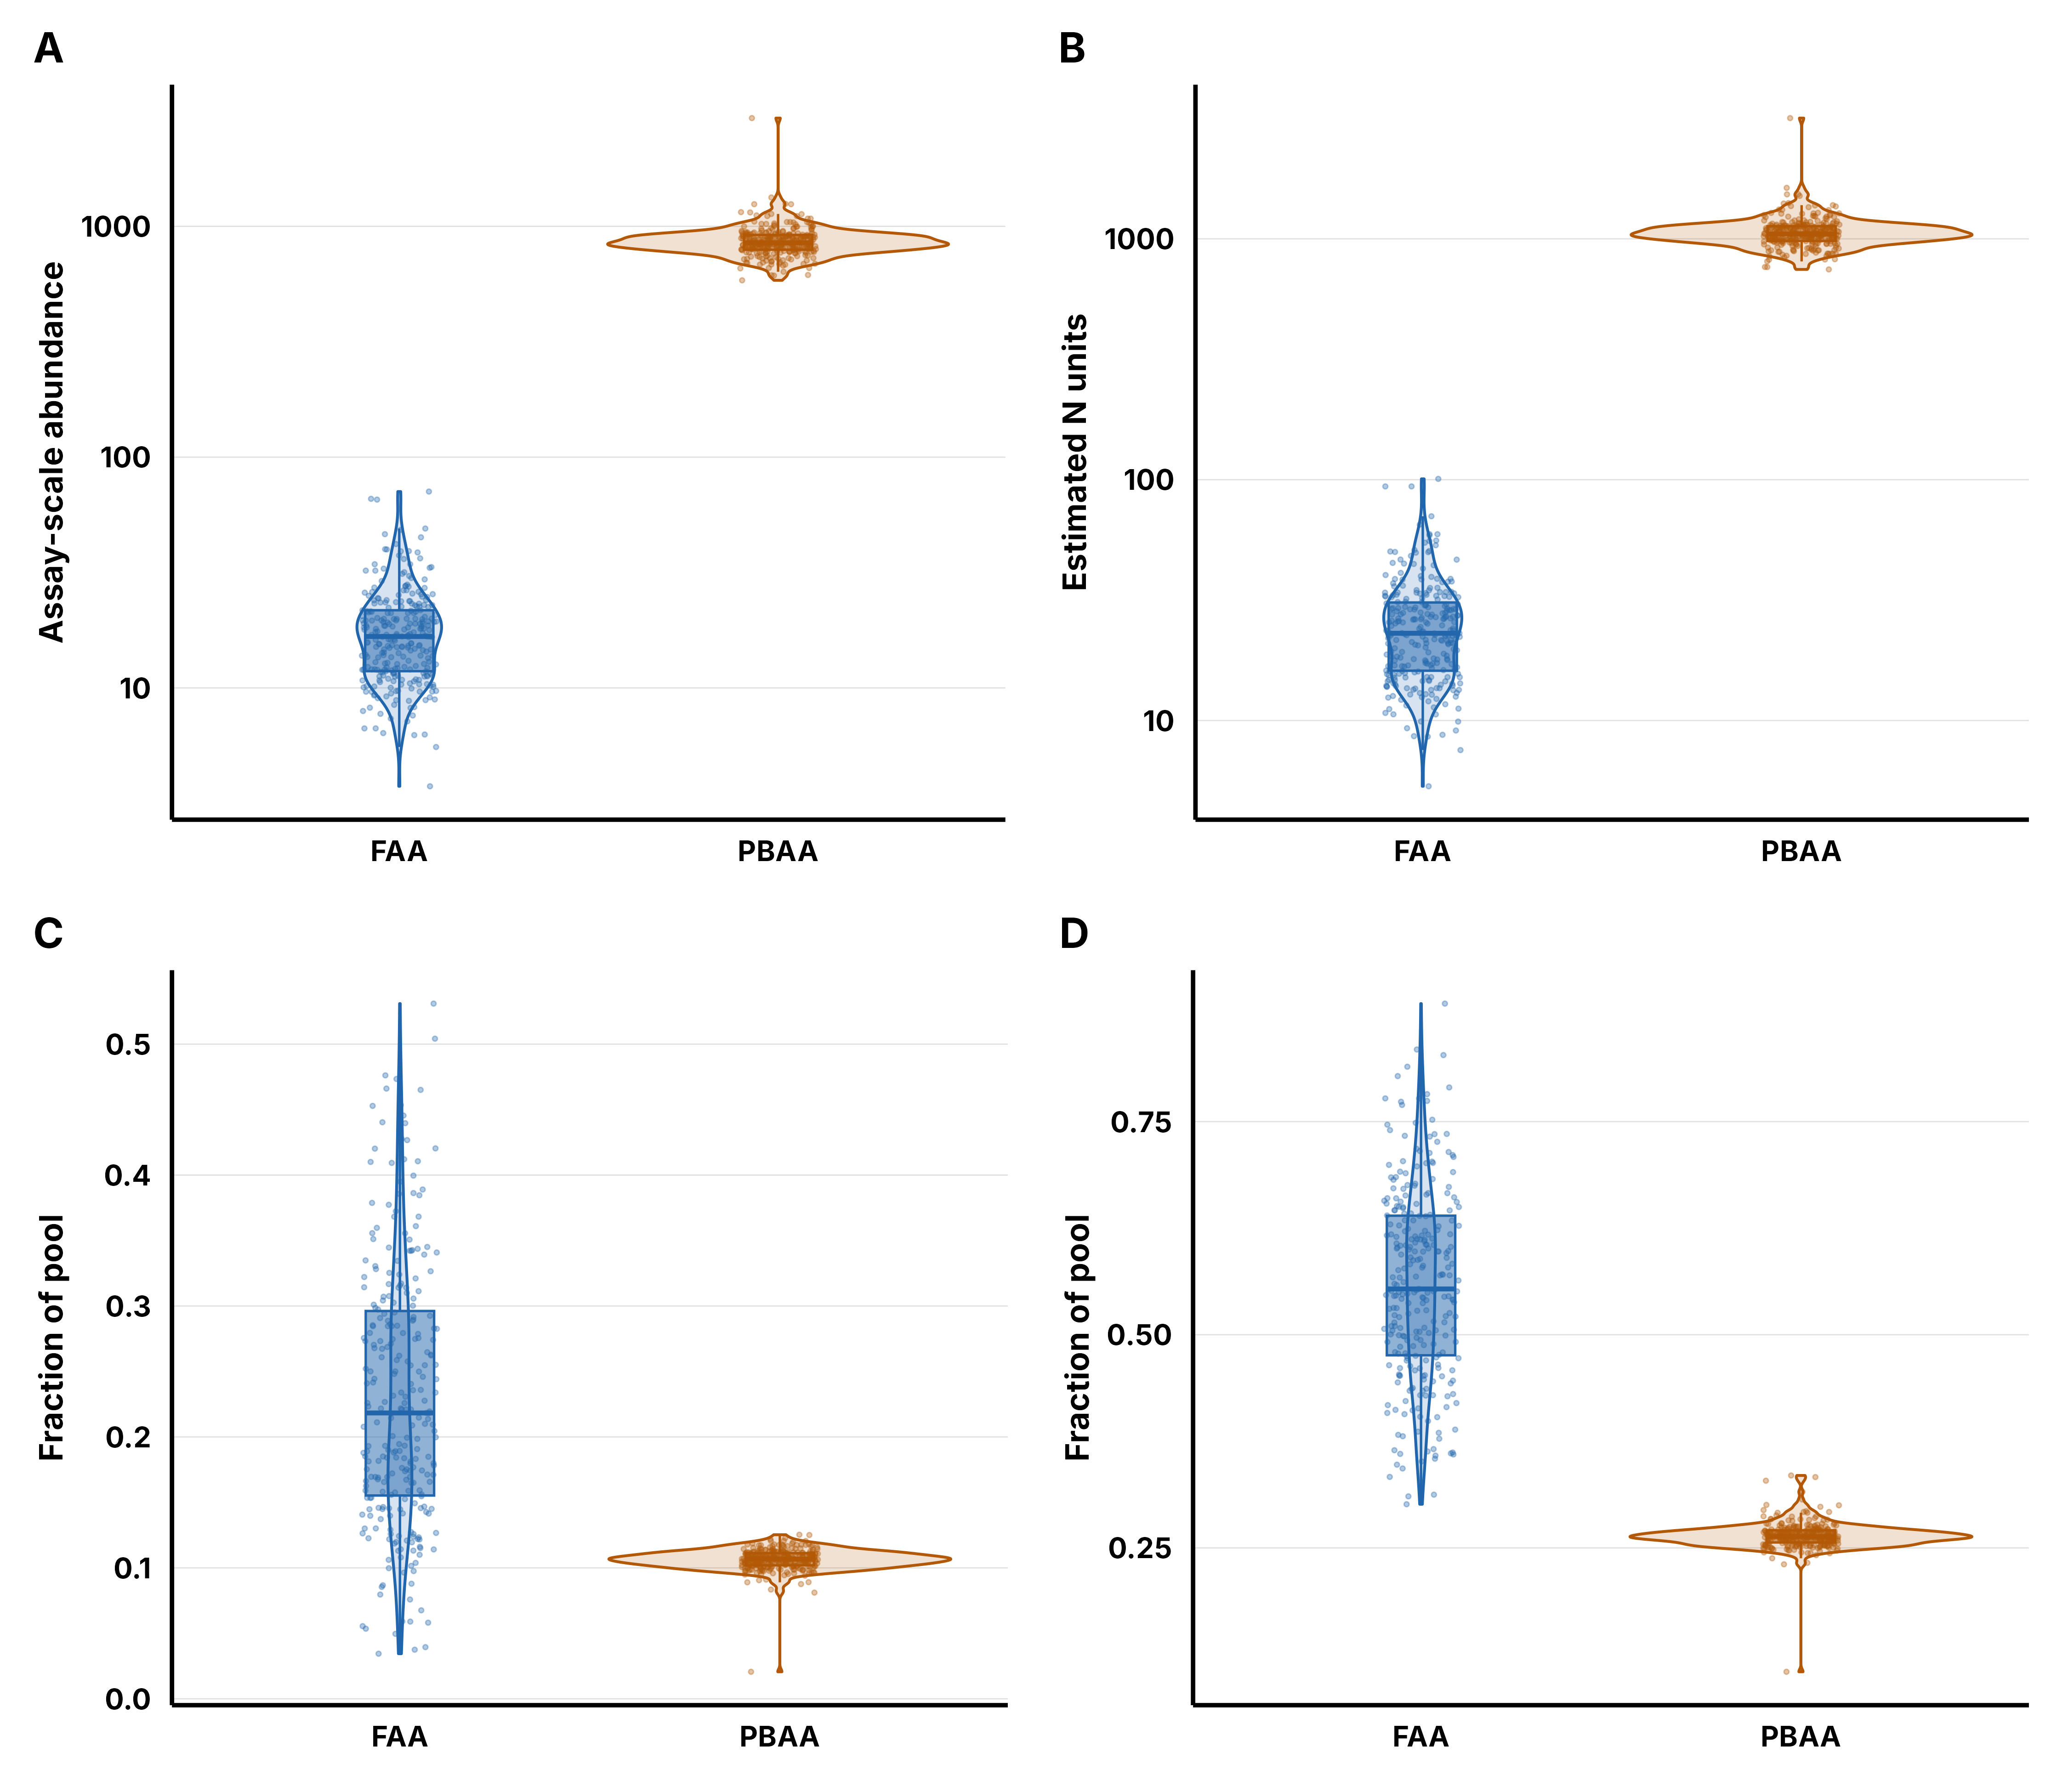
\includegraphics[width=\textwidth]{figures/SuppFig3_FAA_vs_PBAA_pools.png}
\caption*{\textbf{Supplemental Figure S3.} \textbf{Free (FAA) and protein-bound (PBAA) amino acid pools across matched Goodman--Buckler lines ($n = 279$)}. \textbf{(A)}, Total amino acid pool. \textbf{(B)}, Amino acid-derived N proxy, with each amino acid weighted by its number of N atoms (Asx and Glx, unresolved after acid
    hydrolysis, at 1.5 N). \textbf{(C)}, Proline fraction. \textbf{(D)}, Asx + Glx + basic
    (Arg, Lys, His) fraction. Fractions use matched denominators: free Asp + Asn and Glu + Gln
    are combined, and glycine, tryptophan and cysteine are excluded from the free-pool total. Violins show the distribution across lines and boxes the median and interquartile range.}
\end{figure}
\clearpage

\begin{figure}[p]
\centering
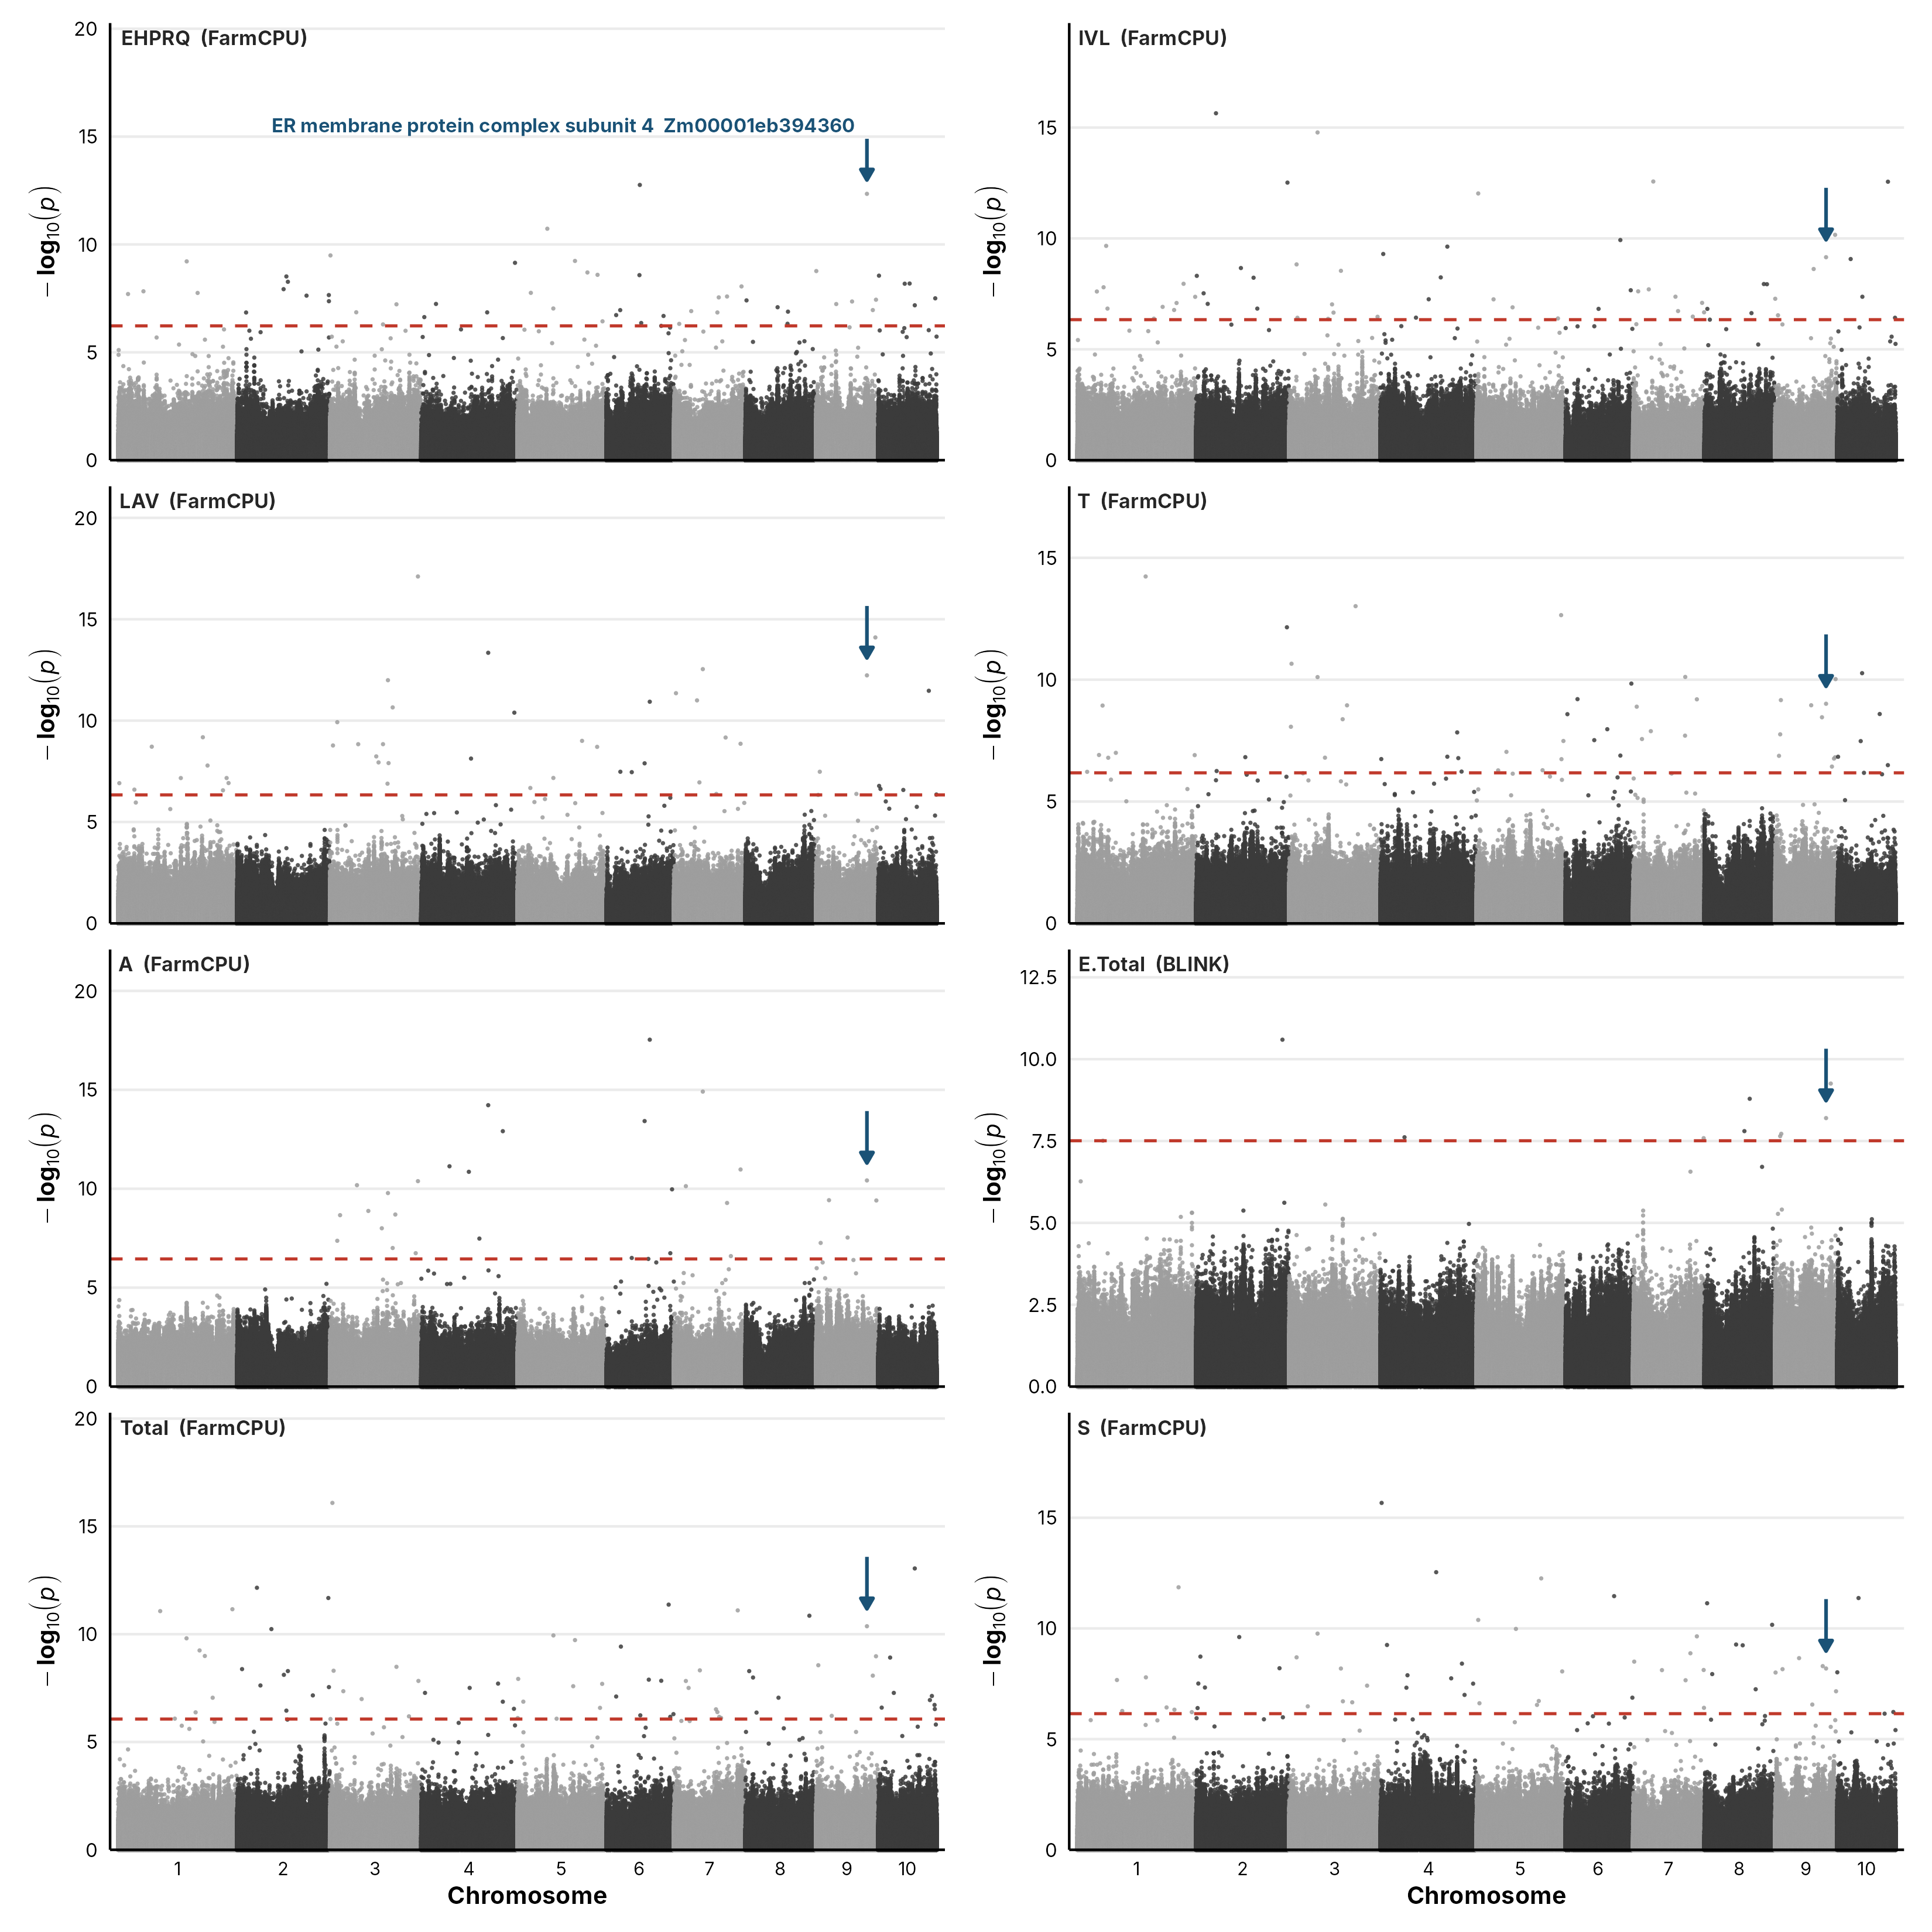
\includegraphics[width=0.82\textwidth]{figures/SuppFig_amino_chr9_locus_manhattan.png}
\caption*{\textbf{Supplemental Figure S4.} \textbf{Manhattan plots for a locus on chromosome 9 associated with nine amino acid phenotypes.} Eight phenotypes had an FDR-significant association near \textit{Zm00001eb394360} (ER membrane protein complex subunit 4; chr9:133,919,123--133,923,877); \textit{N.E} ($P = 1.1 \times 10^{-7}$) is omitted. Four SNPs spanning 13 kb, from the 3$'$ end of \textit{Zm00001eb394360} to the 5$'$ end of \textit{Zm00001eb394380} (rhomboid-like protein 19), are significant for \textit{A}, \textit{LAV}, \textit{IVL}, \textit{T}, \textit{S}, \textit{Total} and \textit{E.Total}, and two further SNPs are significant for \textit{EHPRQ} and \textit{N.E}. Dashed red lines indicate the 5\% Benjamini--Hochberg FDR threshold. The model for each phenotype is in parentheses.}
\end{figure}
\clearpage

\begin{figure}[p]
\centering
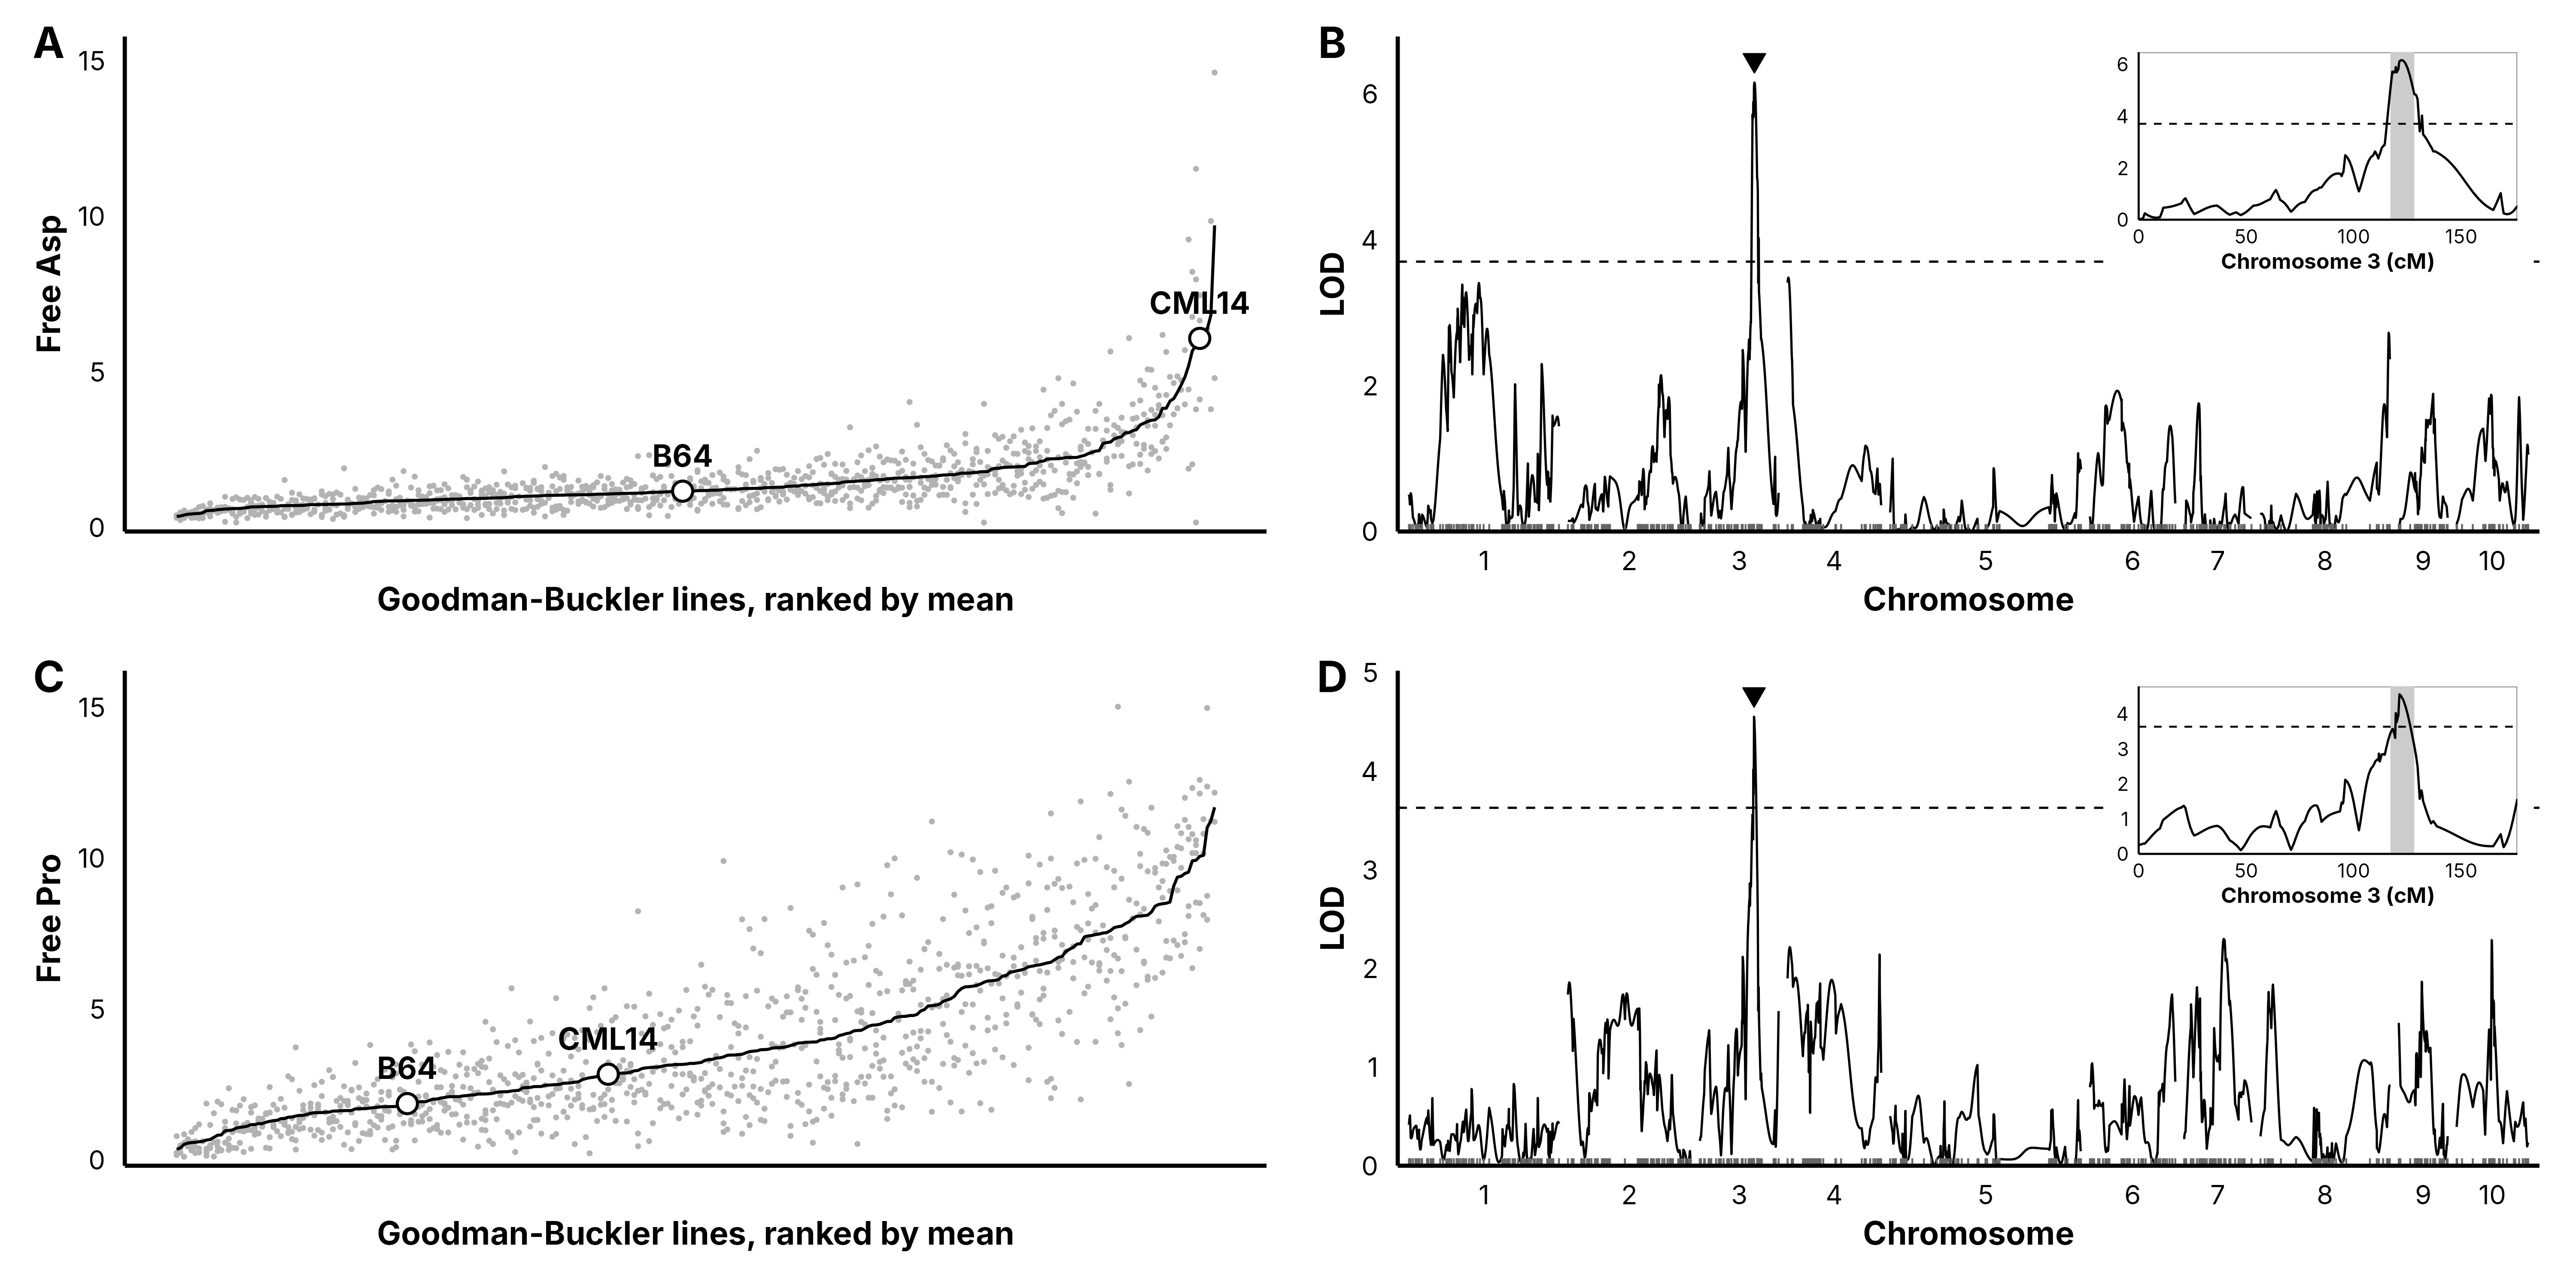
\includegraphics[width=\textwidth]{figures/SuppFig_QTL_Asp_Pro_panel.png}
\caption*{\textbf{Supplemental Figure S5.} \textbf{Free Asp and Pro map to the same QTL on chromosome 3 in the B64 $\times$ CML14 population.} \textbf{(A, C)} Free Asp (A) and Pro (C) in the Goodman--Buckler panel (nmol~$\mu$g$^{-1}$), with lines ranked by their mean. Open circles mark B64 and CML14. \textbf{(B, D)} Genome-wide LOD scores for free Asp (B) and Pro (D) in the B64 $\times$ CML14 F$_{2:3}$ population. Dashed lines show the genome-wide threshold ($\alpha = 0.05$, 1,000 permutations). The triangle marks the chromosome 3 peak, and the inset shows chromosome 3 with the overlap of the Asp and Pro 1.5-LOD support intervals shaded.}
\end{figure}
\clearpage

\begin{figure}[p]
\centering
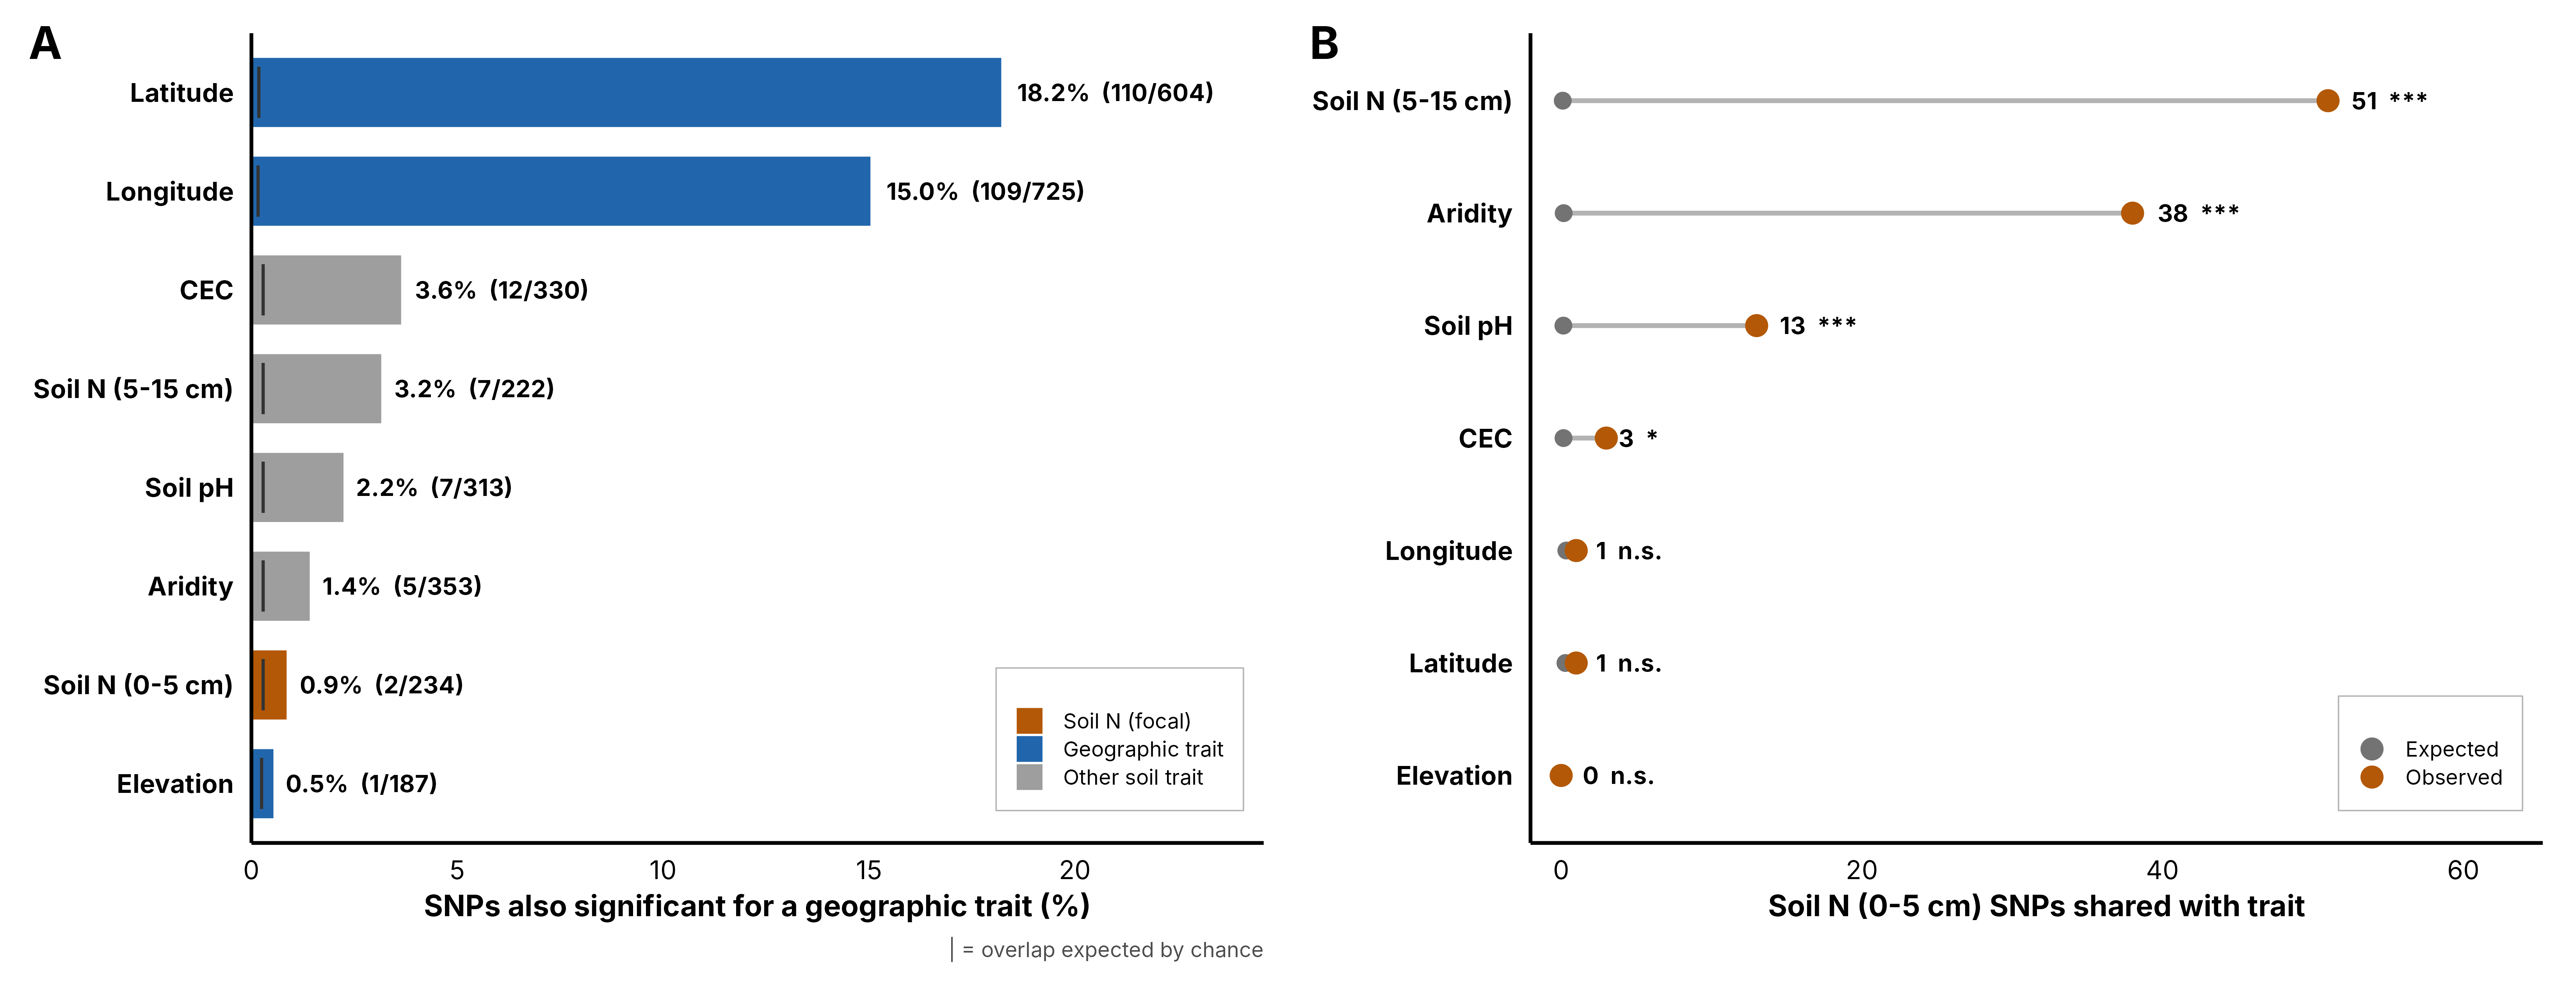
\includegraphics[width=\textwidth]{figures/SuppFig_soilN_specificity.png}
\caption*{\textbf{Supplemental Figure S6.} \textbf{Overlap of soil-N associations with other environmental GWAS.}
  Each variable was scanned with MLM, BLINK and FarmCPU; a SNP counts as
  significant for a variable if it reaches 5\% FDR in any model.
  \textbf{(A)} Percentage of each variable's significant SNPs that are also significant for a
  geographic variable (latitude, longitude, elevation; the variable itself excluded). Vertical
  ticks, percentage expected by chance.
  \textbf{(B)} SNPs shared between soil N (0--5~cm) and each other variable: observed (orange)
  vs.\ expected (gray). One-sided hypergeometric test, $M = 495{,}755$:
  *\,$P<0.05$; **\,$P<10^{-5}$; ***\,$P<10^{-20}$; n.s., not significant.}
\end{figure}
\clearpage

\begin{figure}[p]
\centering
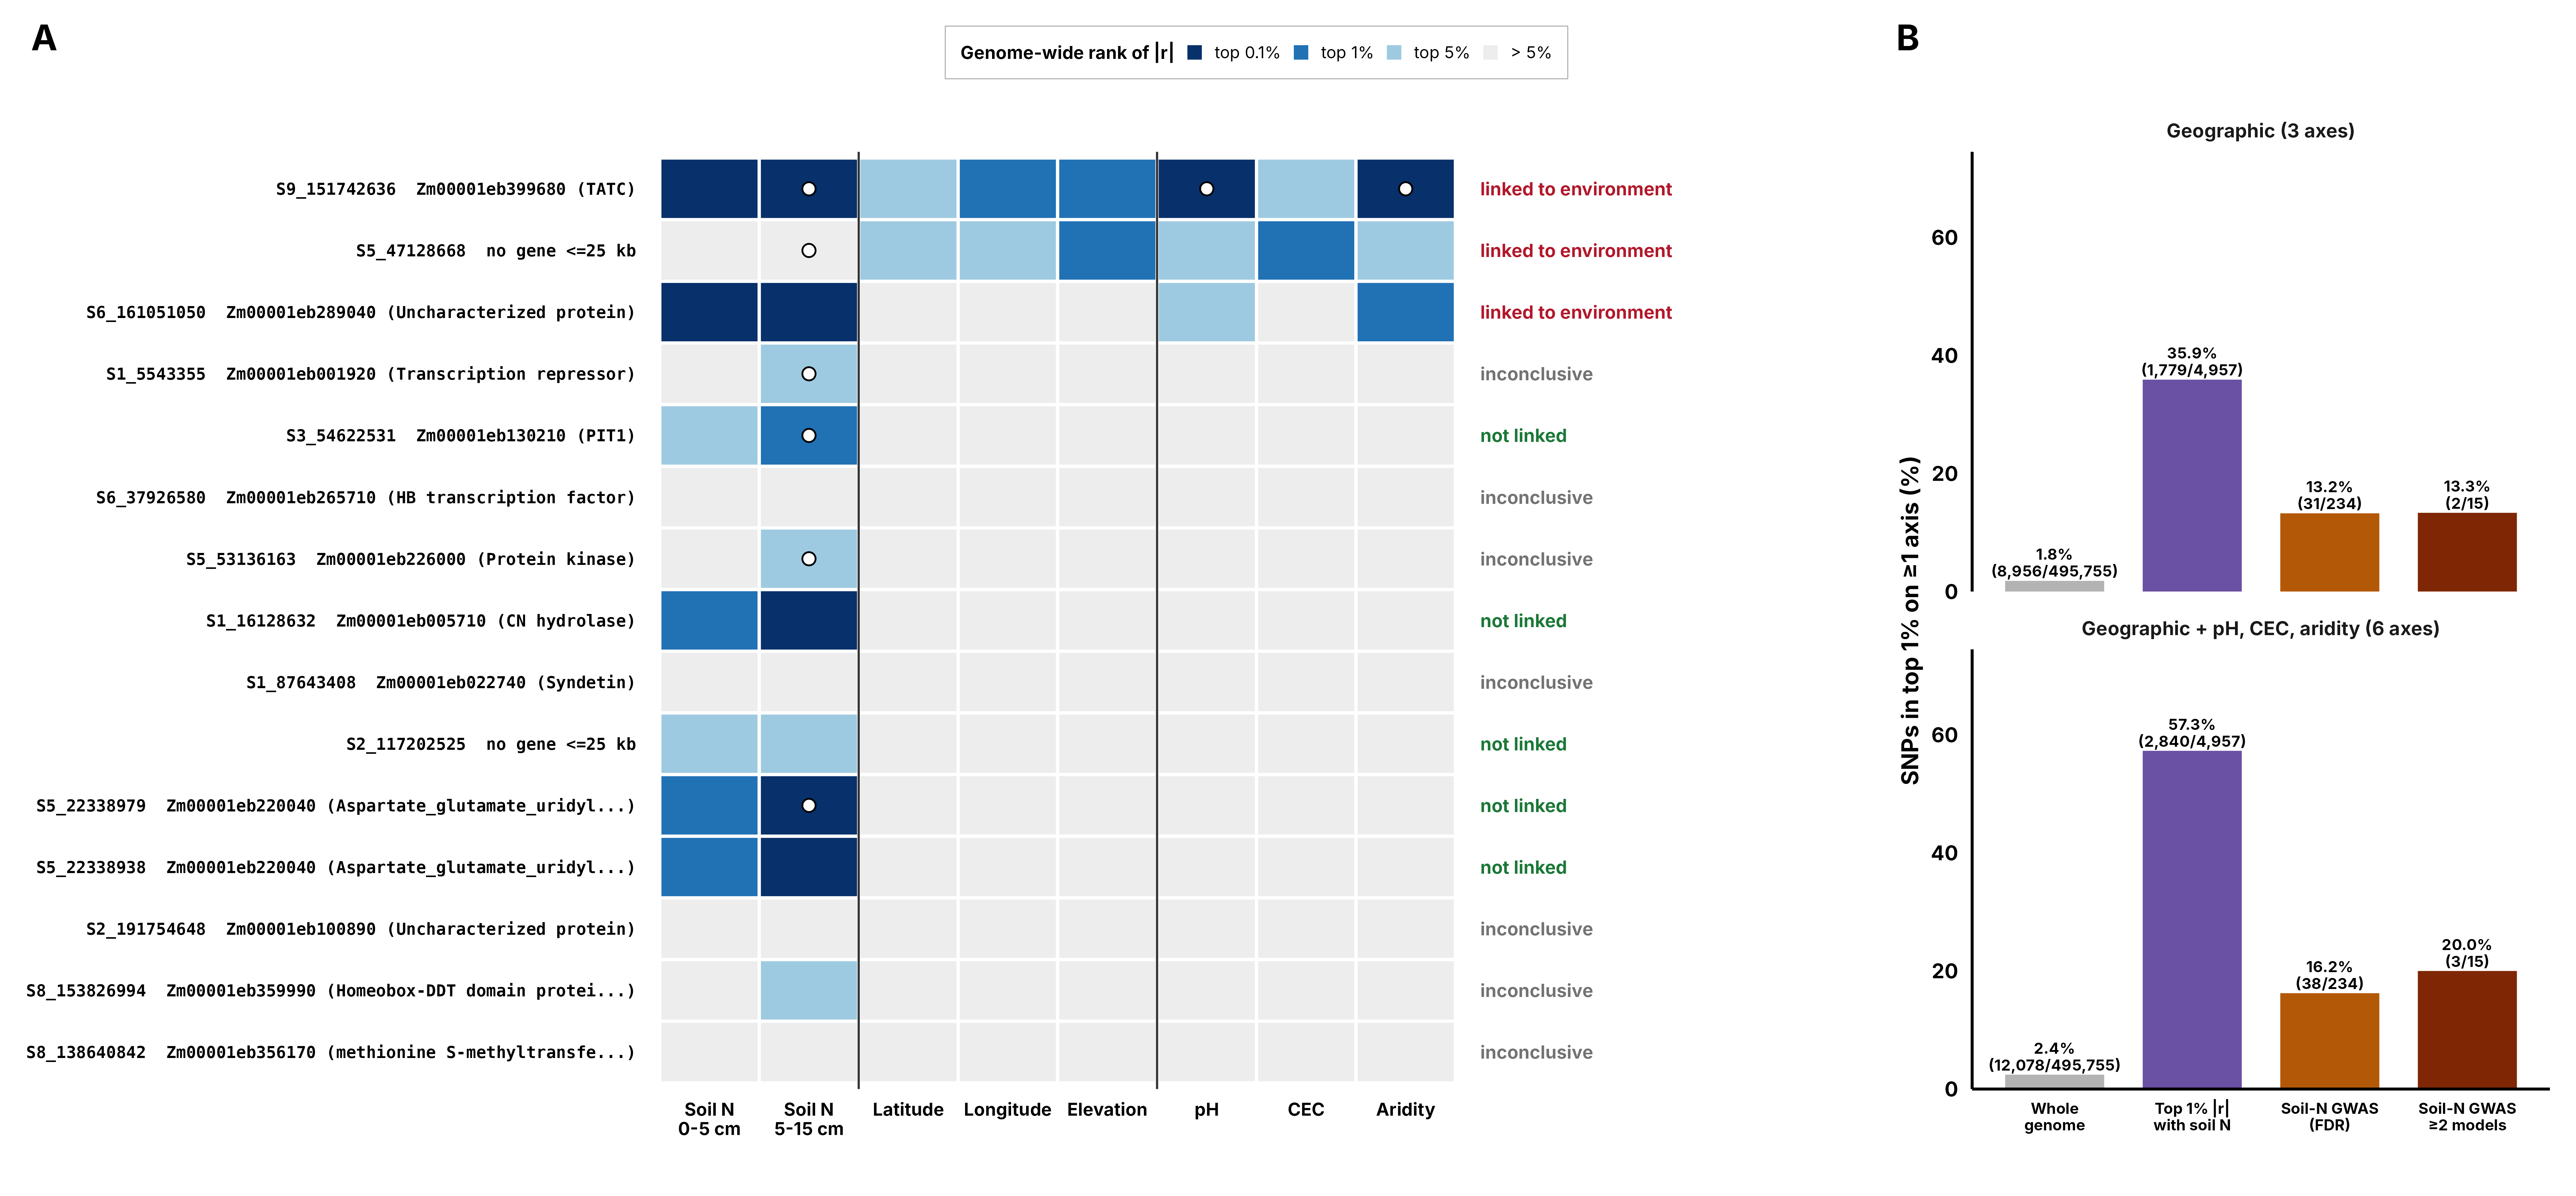
\includegraphics[width=\textwidth]{figures/SuppFig_soilN_geno_env_correlation.png}
\caption*{\textbf{Supplemental Figure S7.} \textbf{Genotype--environment correlation test for the soil-N SNPs.}
  We computed the Pearson correlation ($r$) between the SNP's genotype
  (0, 1 or 2 copies of the allele) and each site variable across 3,107 accessions, then ranked
  every SNP against the whole genome by $|r|$ (e.g.\ ``top 1\%'' = fewer than 1\% of SNPs
  correlate more strongly with that variable).
  \textbf{(A)} The 15 soil-N SNPs significant in at least two GWAS models. Tile color shows the
  genome-wide rank of each SNP's correlation with each variable. Open circles mark SNPs that were
  also significant (5\% FDR) in that variable's own GWAS. Each SNP's call is shown on the right:
  \textit{linked to environment}, its genotype is in the top 1\% of the genome for correlation
  with at least one non-N variable, so its soil-N association cannot be separated from geography
  or climate;
  \textit{not linked}, its genotype correlates strongly with soil N (top 5\%) but not with any
  other variable;
  \textit{inconclusive}, its genotype correlates only weakly with soil N across all accessions
  (outside the top 5\%), so there is no soil-N correlation to compare the other variables
  against. These SNPs were detected only by BLINK and FarmCPU, which test each SNP after
  accounting for population structure and other strongly associated SNPs; this test applies no
  such adjustment and therefore cannot judge them in either direction.
  \textbf{(B)} Expectation test: percentage of SNPs whose genotype is in the top 1\% for at least
  one geographic variable (latitude, longitude, elevation; top) or for at least one of all six
  non-N variables (bottom), for the whole genome, for SNPs in the top 1\% for correlation with
  soil N, and for the soil-N GWAS SNPs.}
\end{figure}
\clearpage

\begin{figure}[p]
\centering
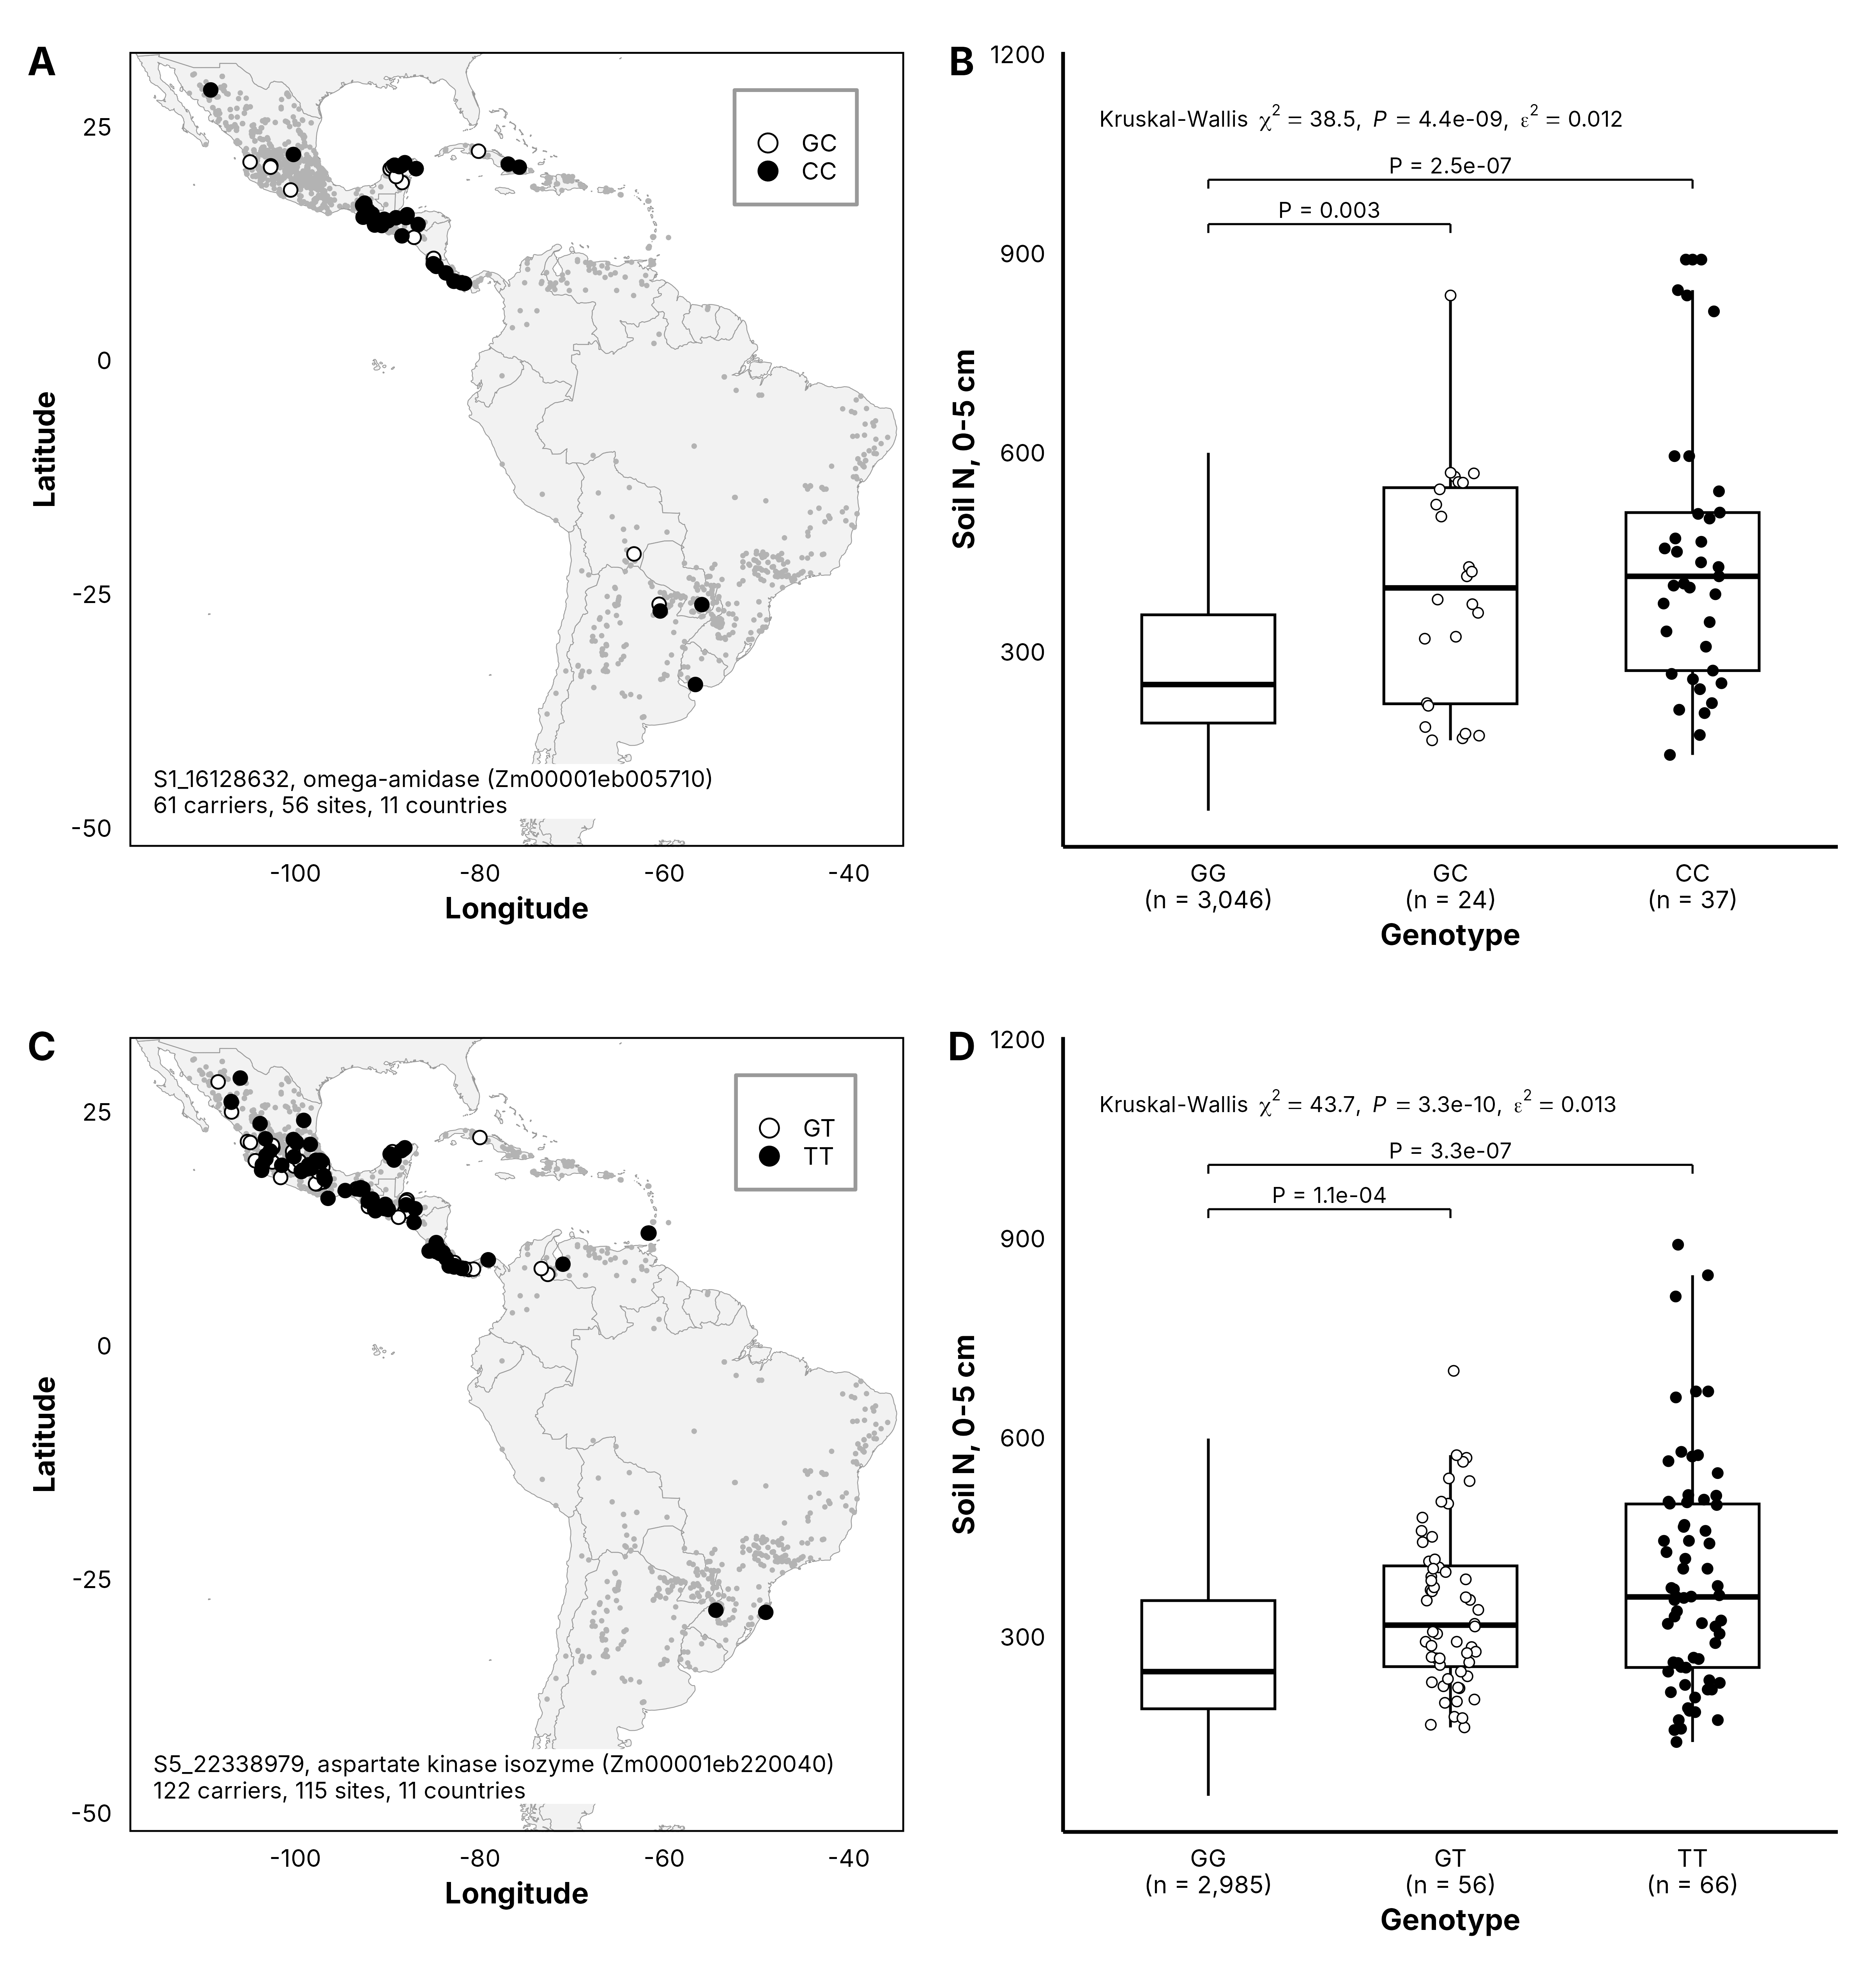
\includegraphics[width=0.85\textwidth]{figures/SuppFig_soilN_focal_allele_geography.png}
\caption*{\textbf{Supplemental Figure S8.} \textbf{Geography and soil N of the two focal soil-N SNPs.} \textbf{(A, B)} S1\_16128632 in the $\omega$-amidase gene \textit{Zm00001eb005710}. \textbf{(C, D)} S5\_22338979 near the aspartate kinase isozyme gene \textit{Zm00001eb220040}. \textbf{(A, C)} Collection sites of the 3,107 landraces. Gray, homozygous for the major allele; white, heterozygous; black, homozygous for the minor allele. Numbers of carriers, independent collection sites, and countries are given in each panel. \textbf{(B, D)} Soil N at 0--5 cm by genotype. Boxes show the median and interquartile range, and points show individual values. Differences among genotypes were tested with a Kruskal--Wallis test ($\varepsilon^2$, effect size), followed by Dunn tests with Holm correction, and only significant pairwise comparisons are shown.}
\end{figure}
\clearpage

\begin{figure}[p]
\centering
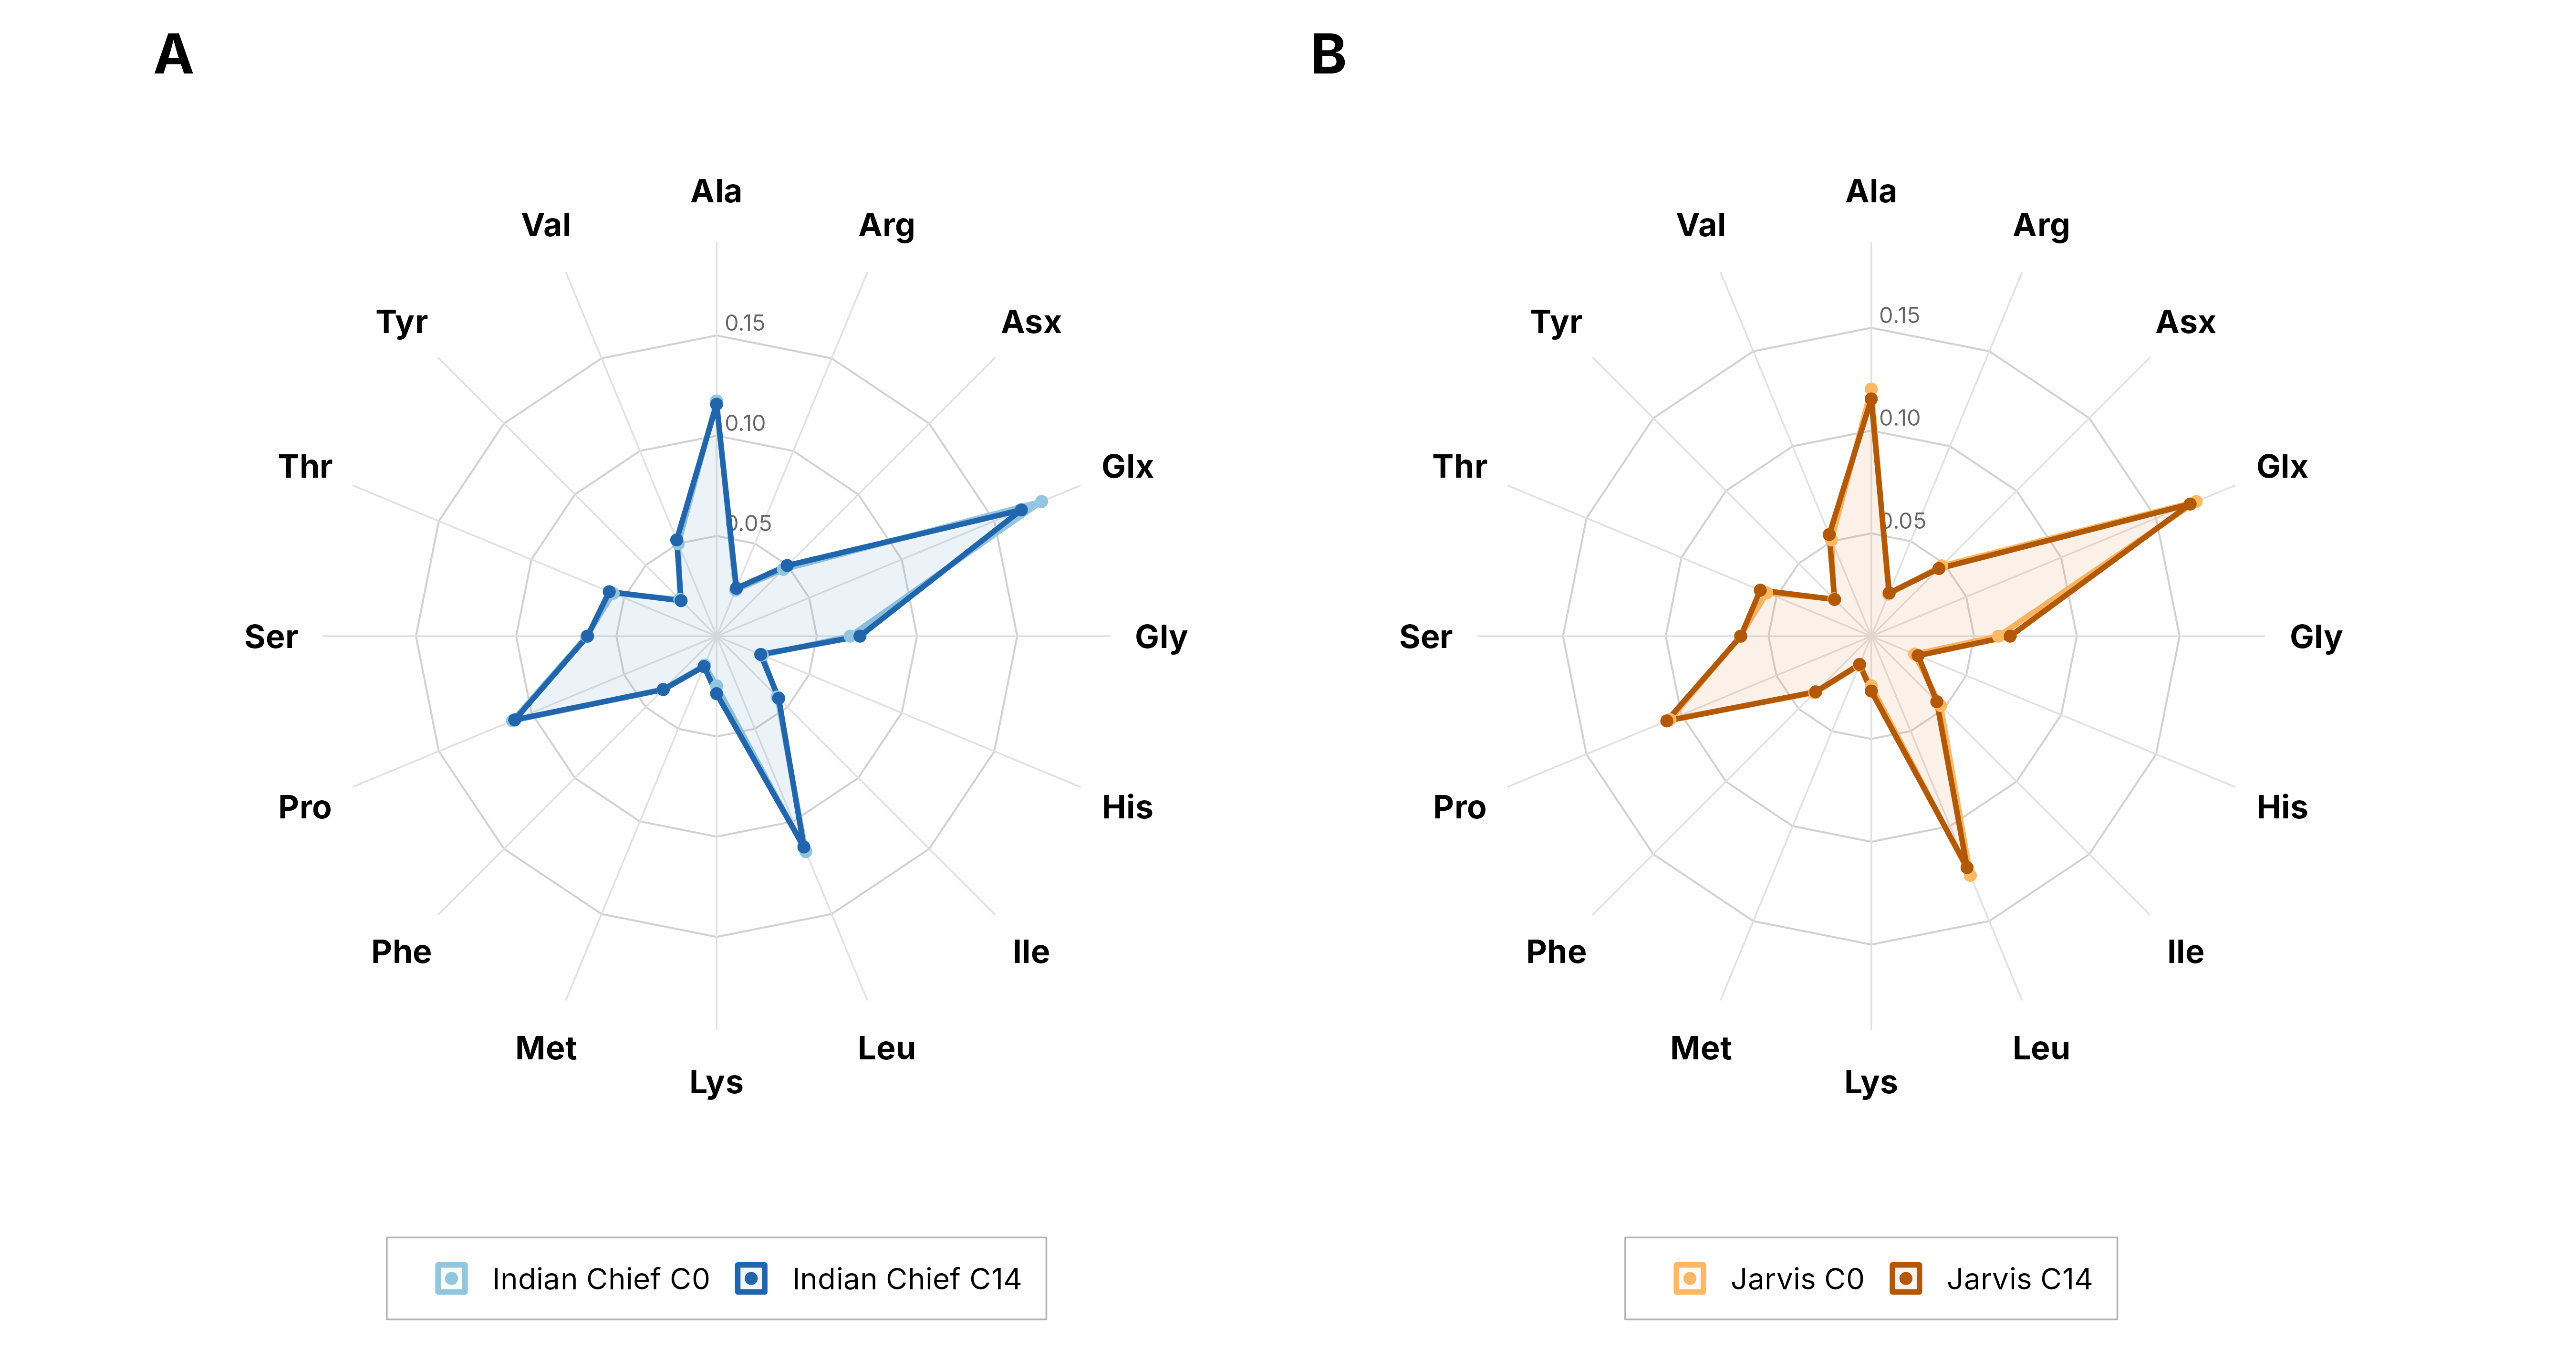
\includegraphics[width=\textwidth]{figures/SuppFig_IC_J_PBAA_composition.png}
\caption*{\textbf{Supplemental Figure S9.} \textbf{Protein-bound amino acid (PBAA) composition in Indian Chief and Jarvis at Cycle 0 (C0) and Cycle 14 (C14).} Mean fraction of each of 16 PBAA in the total PBAA pool, averaged over biological samples, for \textbf{(A)} Indian Chief and \textbf{(B)} Jarvis. Asx and Glx are the combined Asp + Asn and Glu + Gln pools after acid hydrolysis; tryptophan and cysteine are not measured. Rings mark fractions of 0.05, 0.10 and 0.15. No amino acid differed between cycles in either population (two-sided Wilcoxon rank-sum tests, Benjamini--Hochberg-adjusted across the 16 amino acids.}
\end{figure}
\clearpage

\begin{figure}[p]
\centering
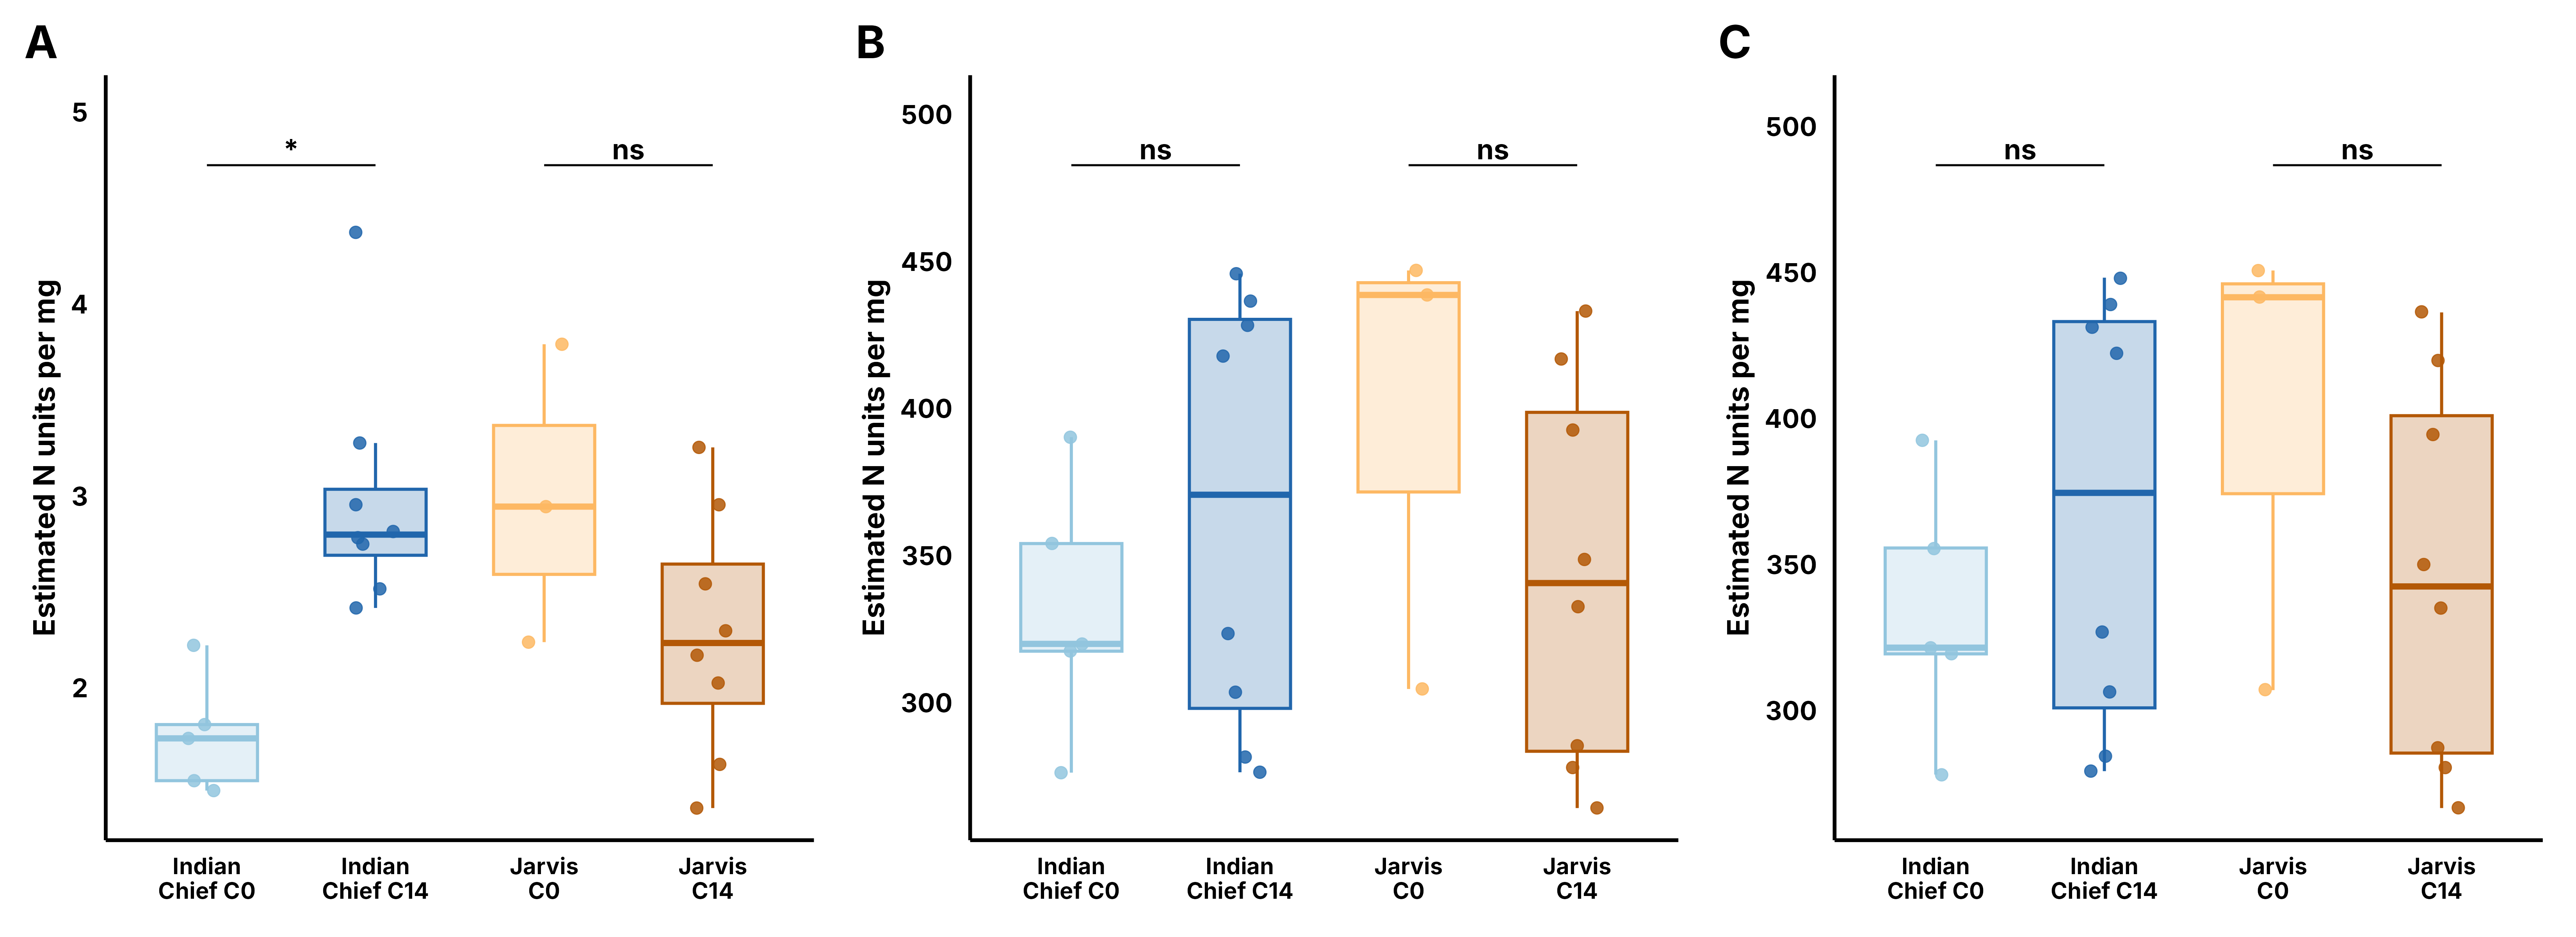
\includegraphics[width=\textwidth]{figures/SuppFig_IC_J_AA_N_pools.png}
\caption*{\textbf{Supplemental Figure S10.} \textbf{Amino acid-derived nitrogen per mg sample in Indian Chief and Jarvis at Cycle 0 (C0) and Cycle~14 (C14).} \textbf{(A)} FAA-derived N, \textbf{(B)} estimated protein-bound amino acid-derived N and \textbf{(C)} estimated total amino acid-derived N (A + B). Each amino acid was weighted by its number of N atoms (Arg 4; His 3; Asn, Gln, Lys and Trp 2; all others 1; protein-bound Asx and Glx 1.5) and divided by sample mass. Points are biological samples (Indian Chief C0 $n = 5$, C14 $n = 8$; Jarvis C0 $n = 3$, C14 $n = 8$); boxes show the median and interquartile range. Brackets show within-population two-sided Wilcoxon rank-sum tests, Benjamini--Hochberg-adjusted across the three measures: * adjusted $P < 0.05$; ns, not significant.}
\end{figure}
\clearpage

\begin{figure}[p]
\centering
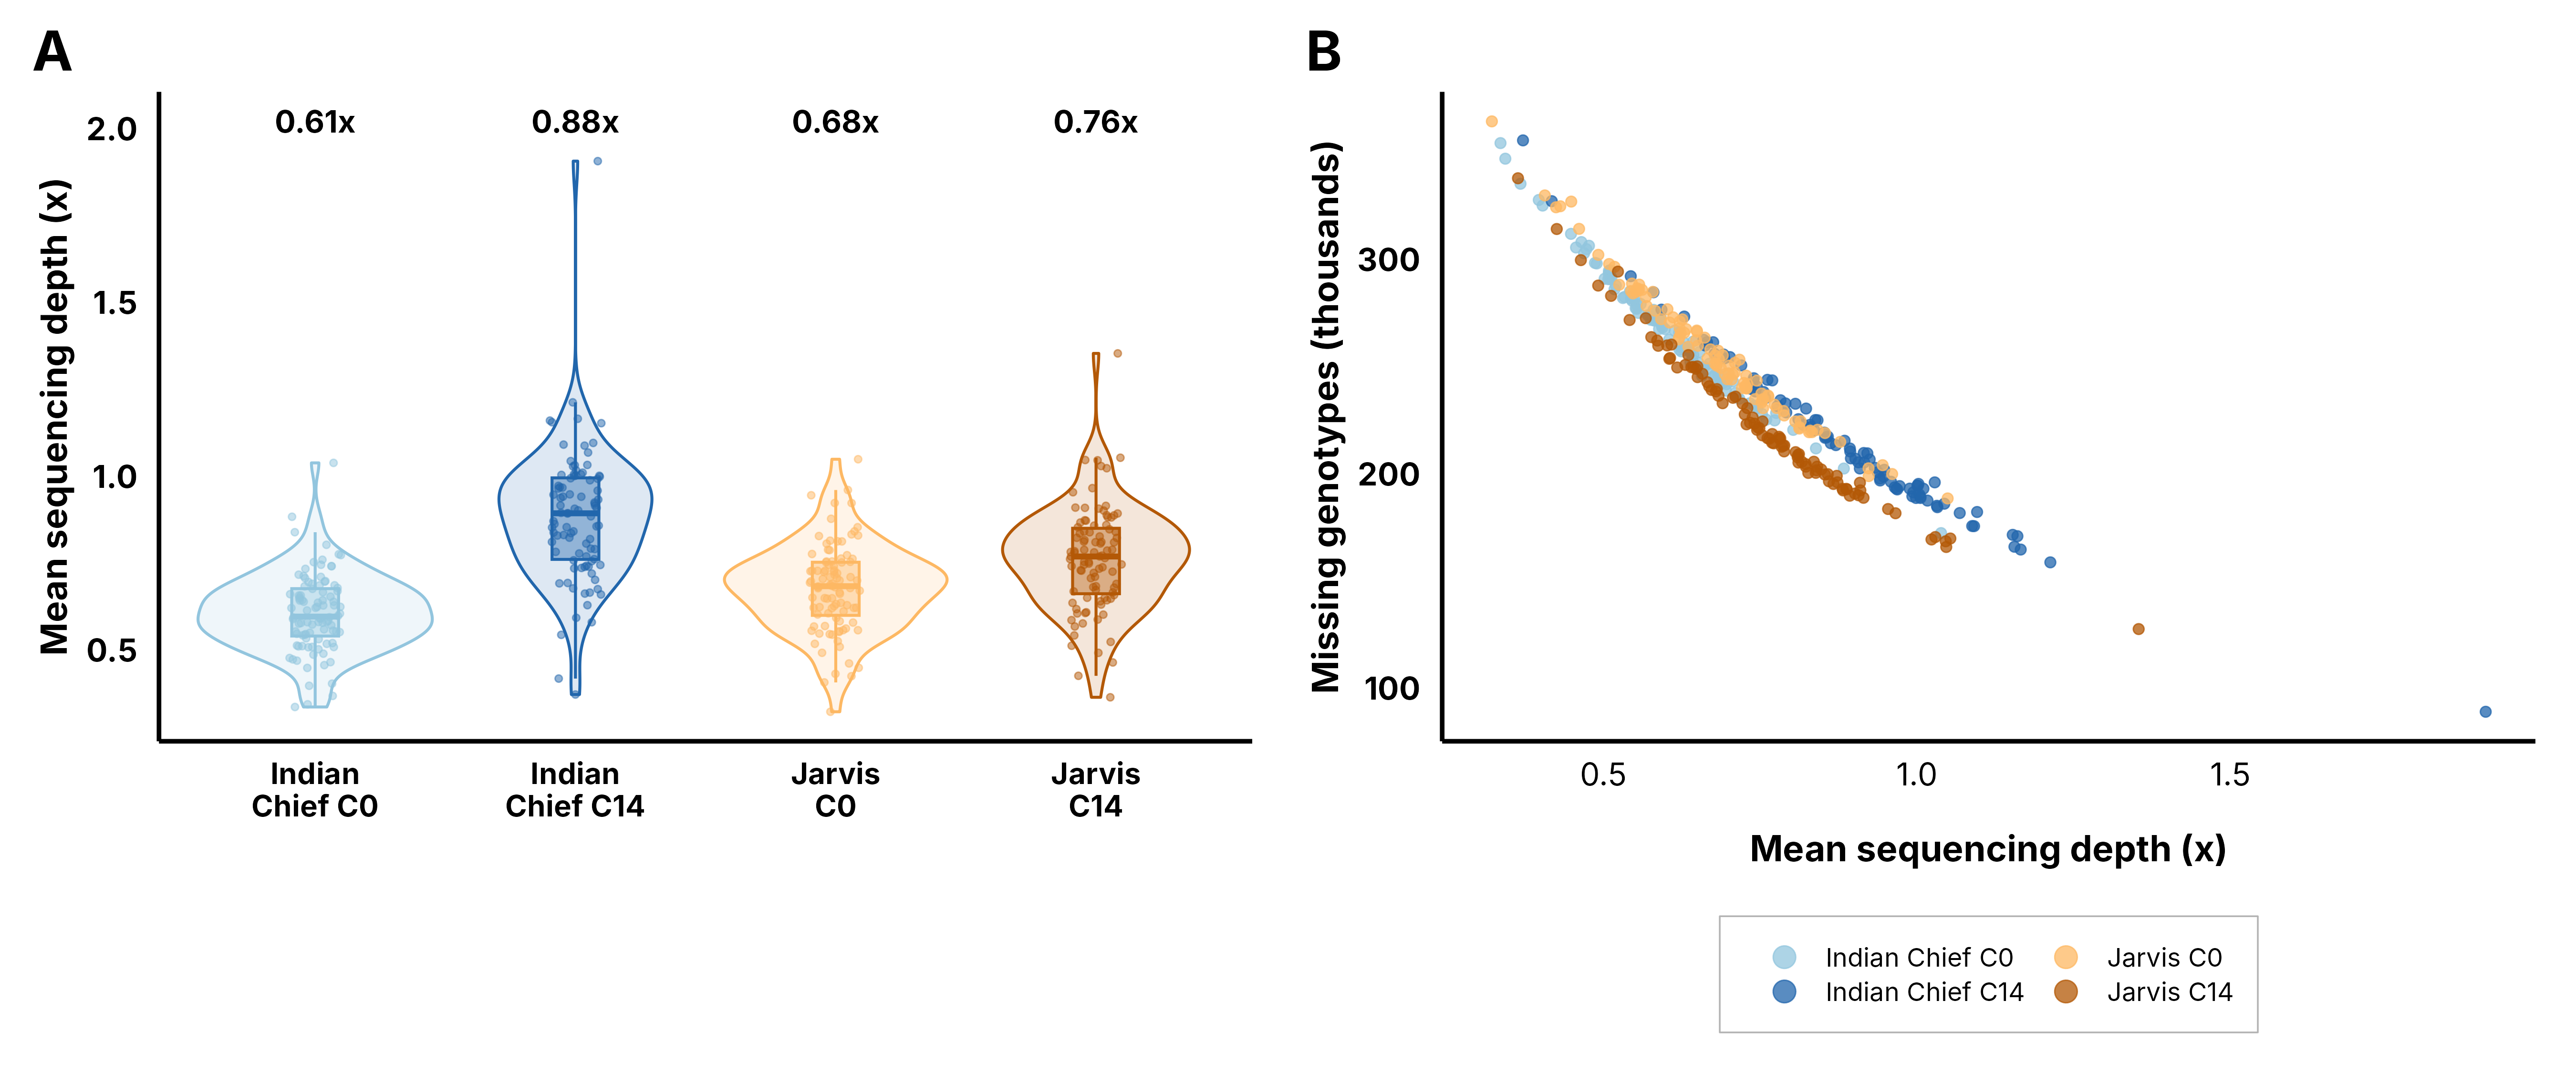
\includegraphics[width=\textwidth]{figures/SuppFig_seq_statistics_sample_level.png}
\caption*{\textbf{Supplemental Figure S11.} \textbf{Per-sample sequencing depth in the Indian Chief and Jarvis skim-sequencing data.} \textbf{(A)} Mean sequencing depth per individual for each population and cycle; numbers give group means. \textbf{(B)} Number of missing genotypes (of 512,667 filtered SNPs) per individual against its mean depth.}
\end{figure}
\clearpage

\begin{figure}[p]
\centering
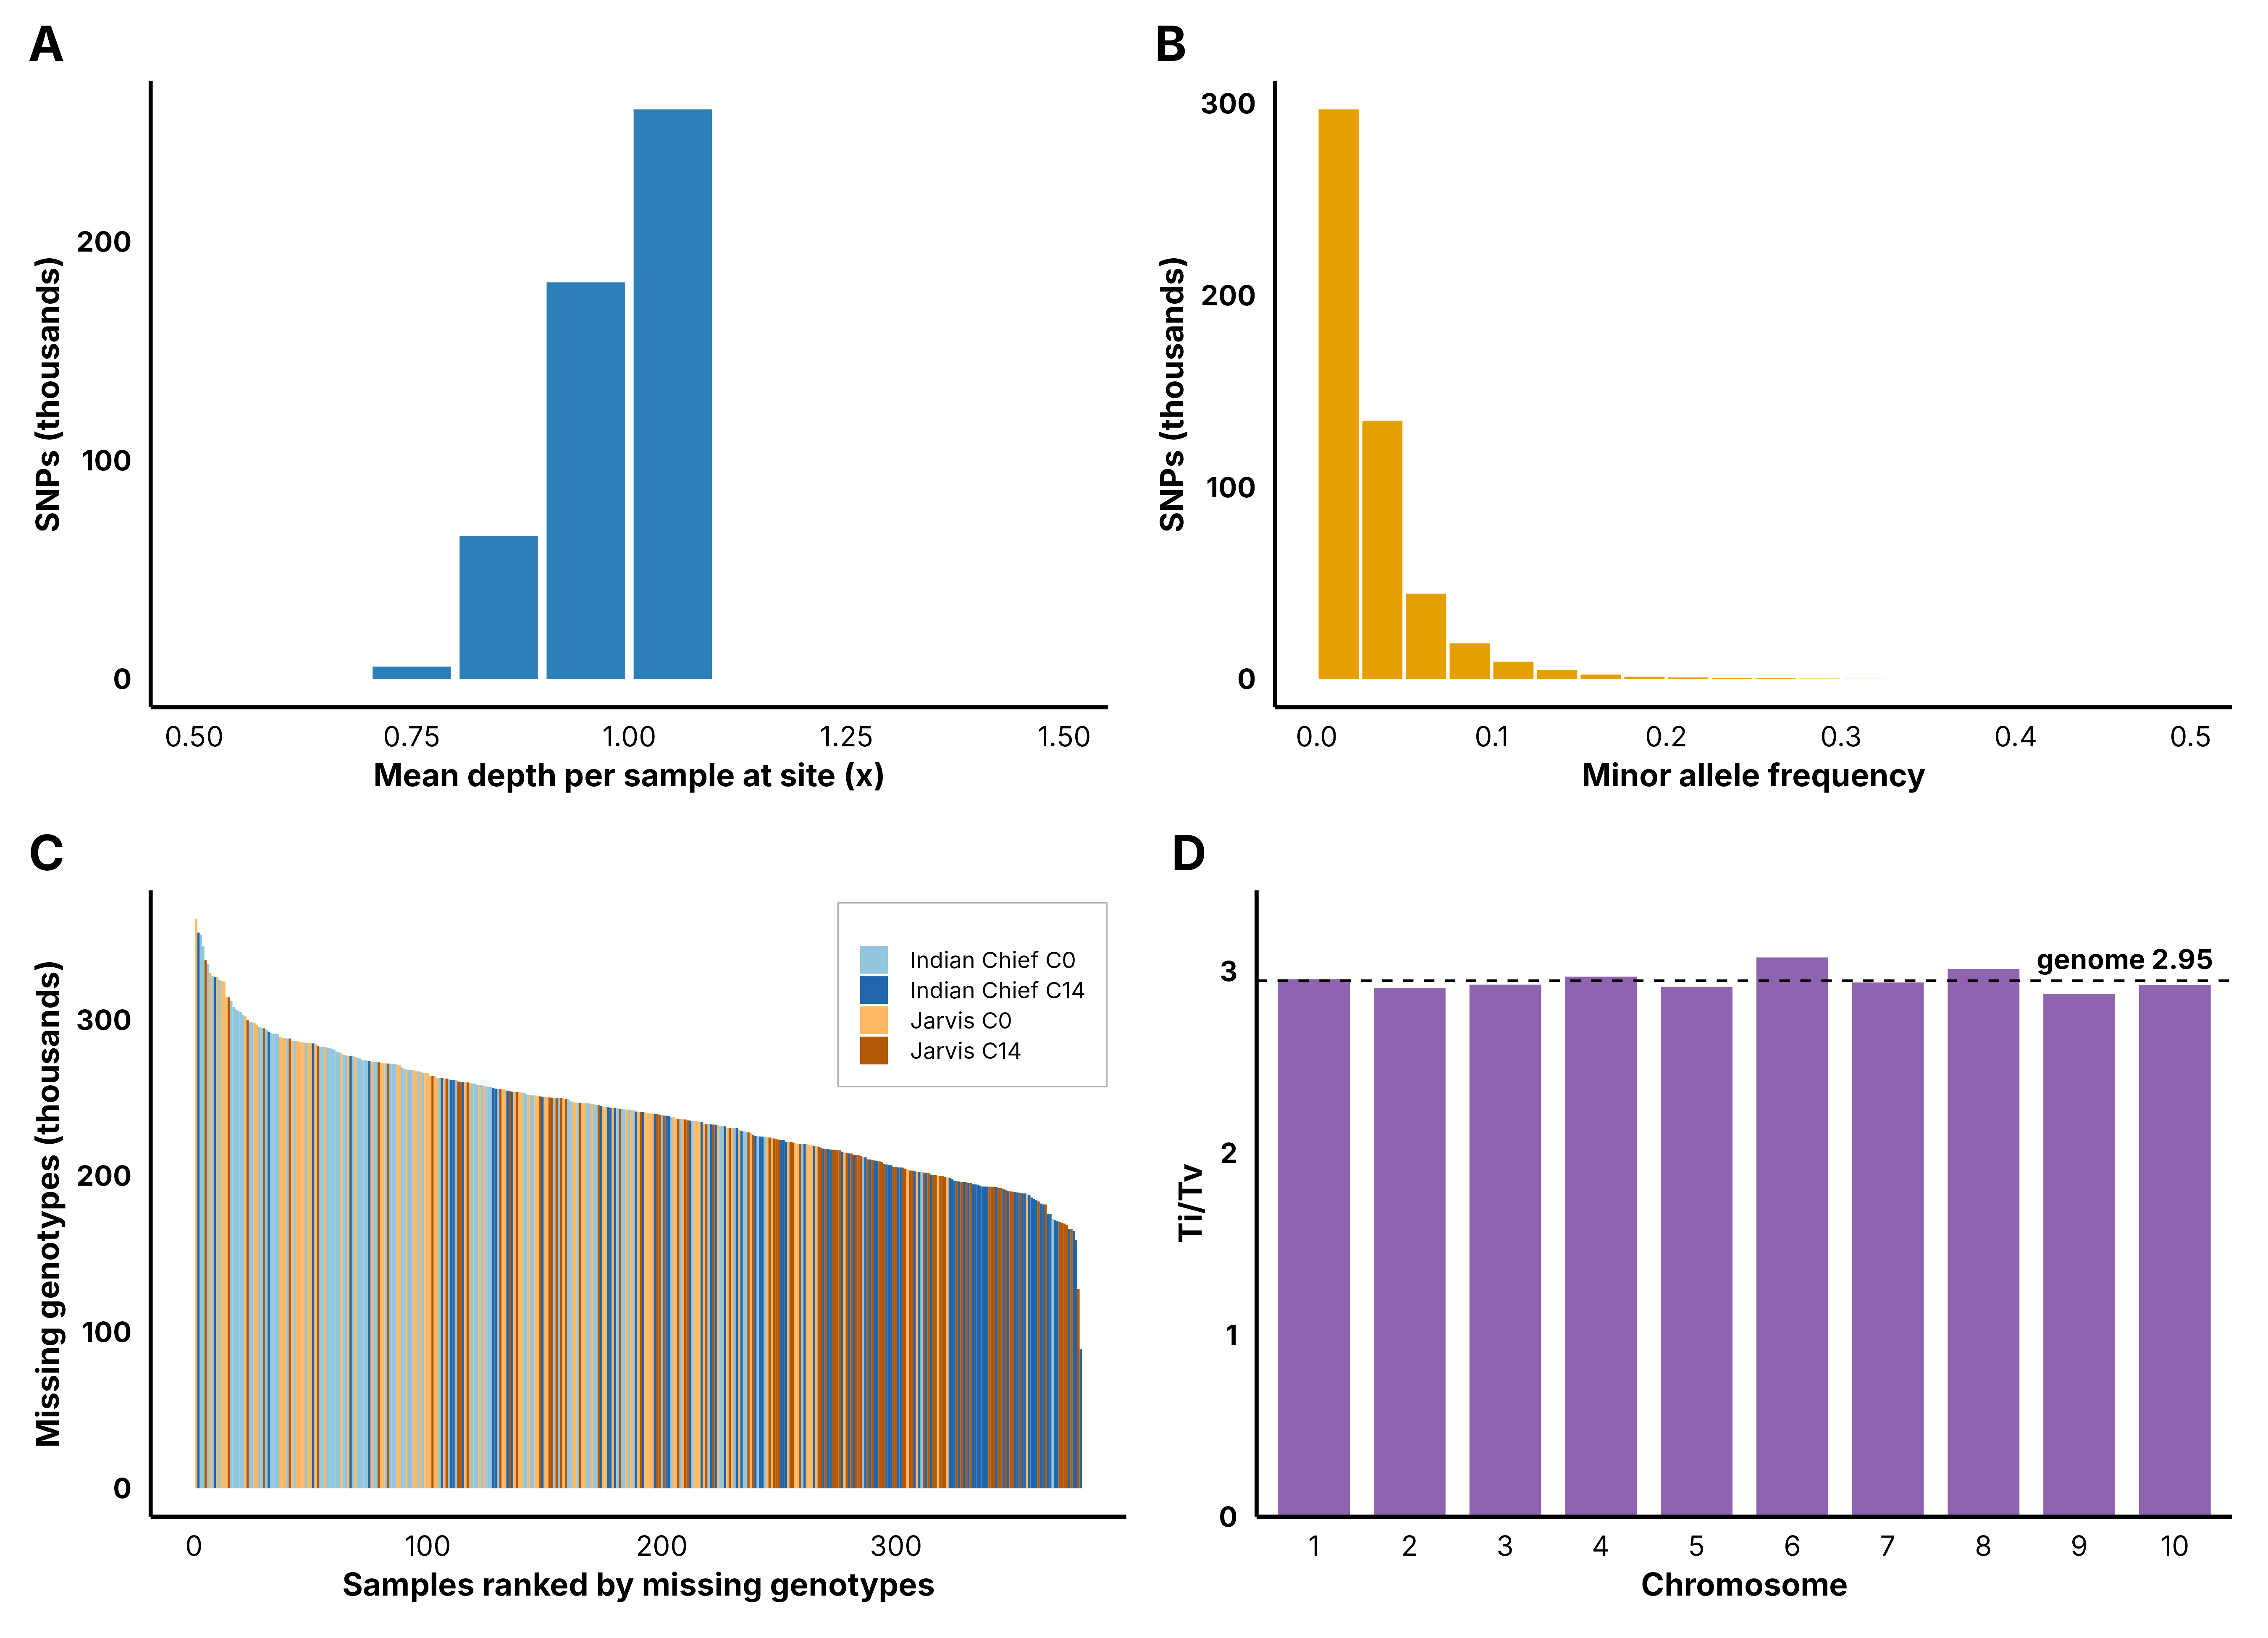
\includegraphics[width=\textwidth]{figures/SuppFig_seq_statistics_variant_level.png}
\caption*{\textbf{Supplemental Figure S12.} \textbf{Quality summaries for the 512,667 filtered SNPs.} \textbf{(A)} Mean depth per individual at each SNP (total site depth divided by 379). \textbf{(B)} Minor allele frequency spectrum, from called genotypes. \textbf{(C)} Missing genotypes per individual, ranked and colored by population and cycle. \textbf{(D)} Transition/transversion ratio by chromosome; dashed line, genome-wide value.}
\end{figure}
\clearpage

\begin{figure}[p]
\centering
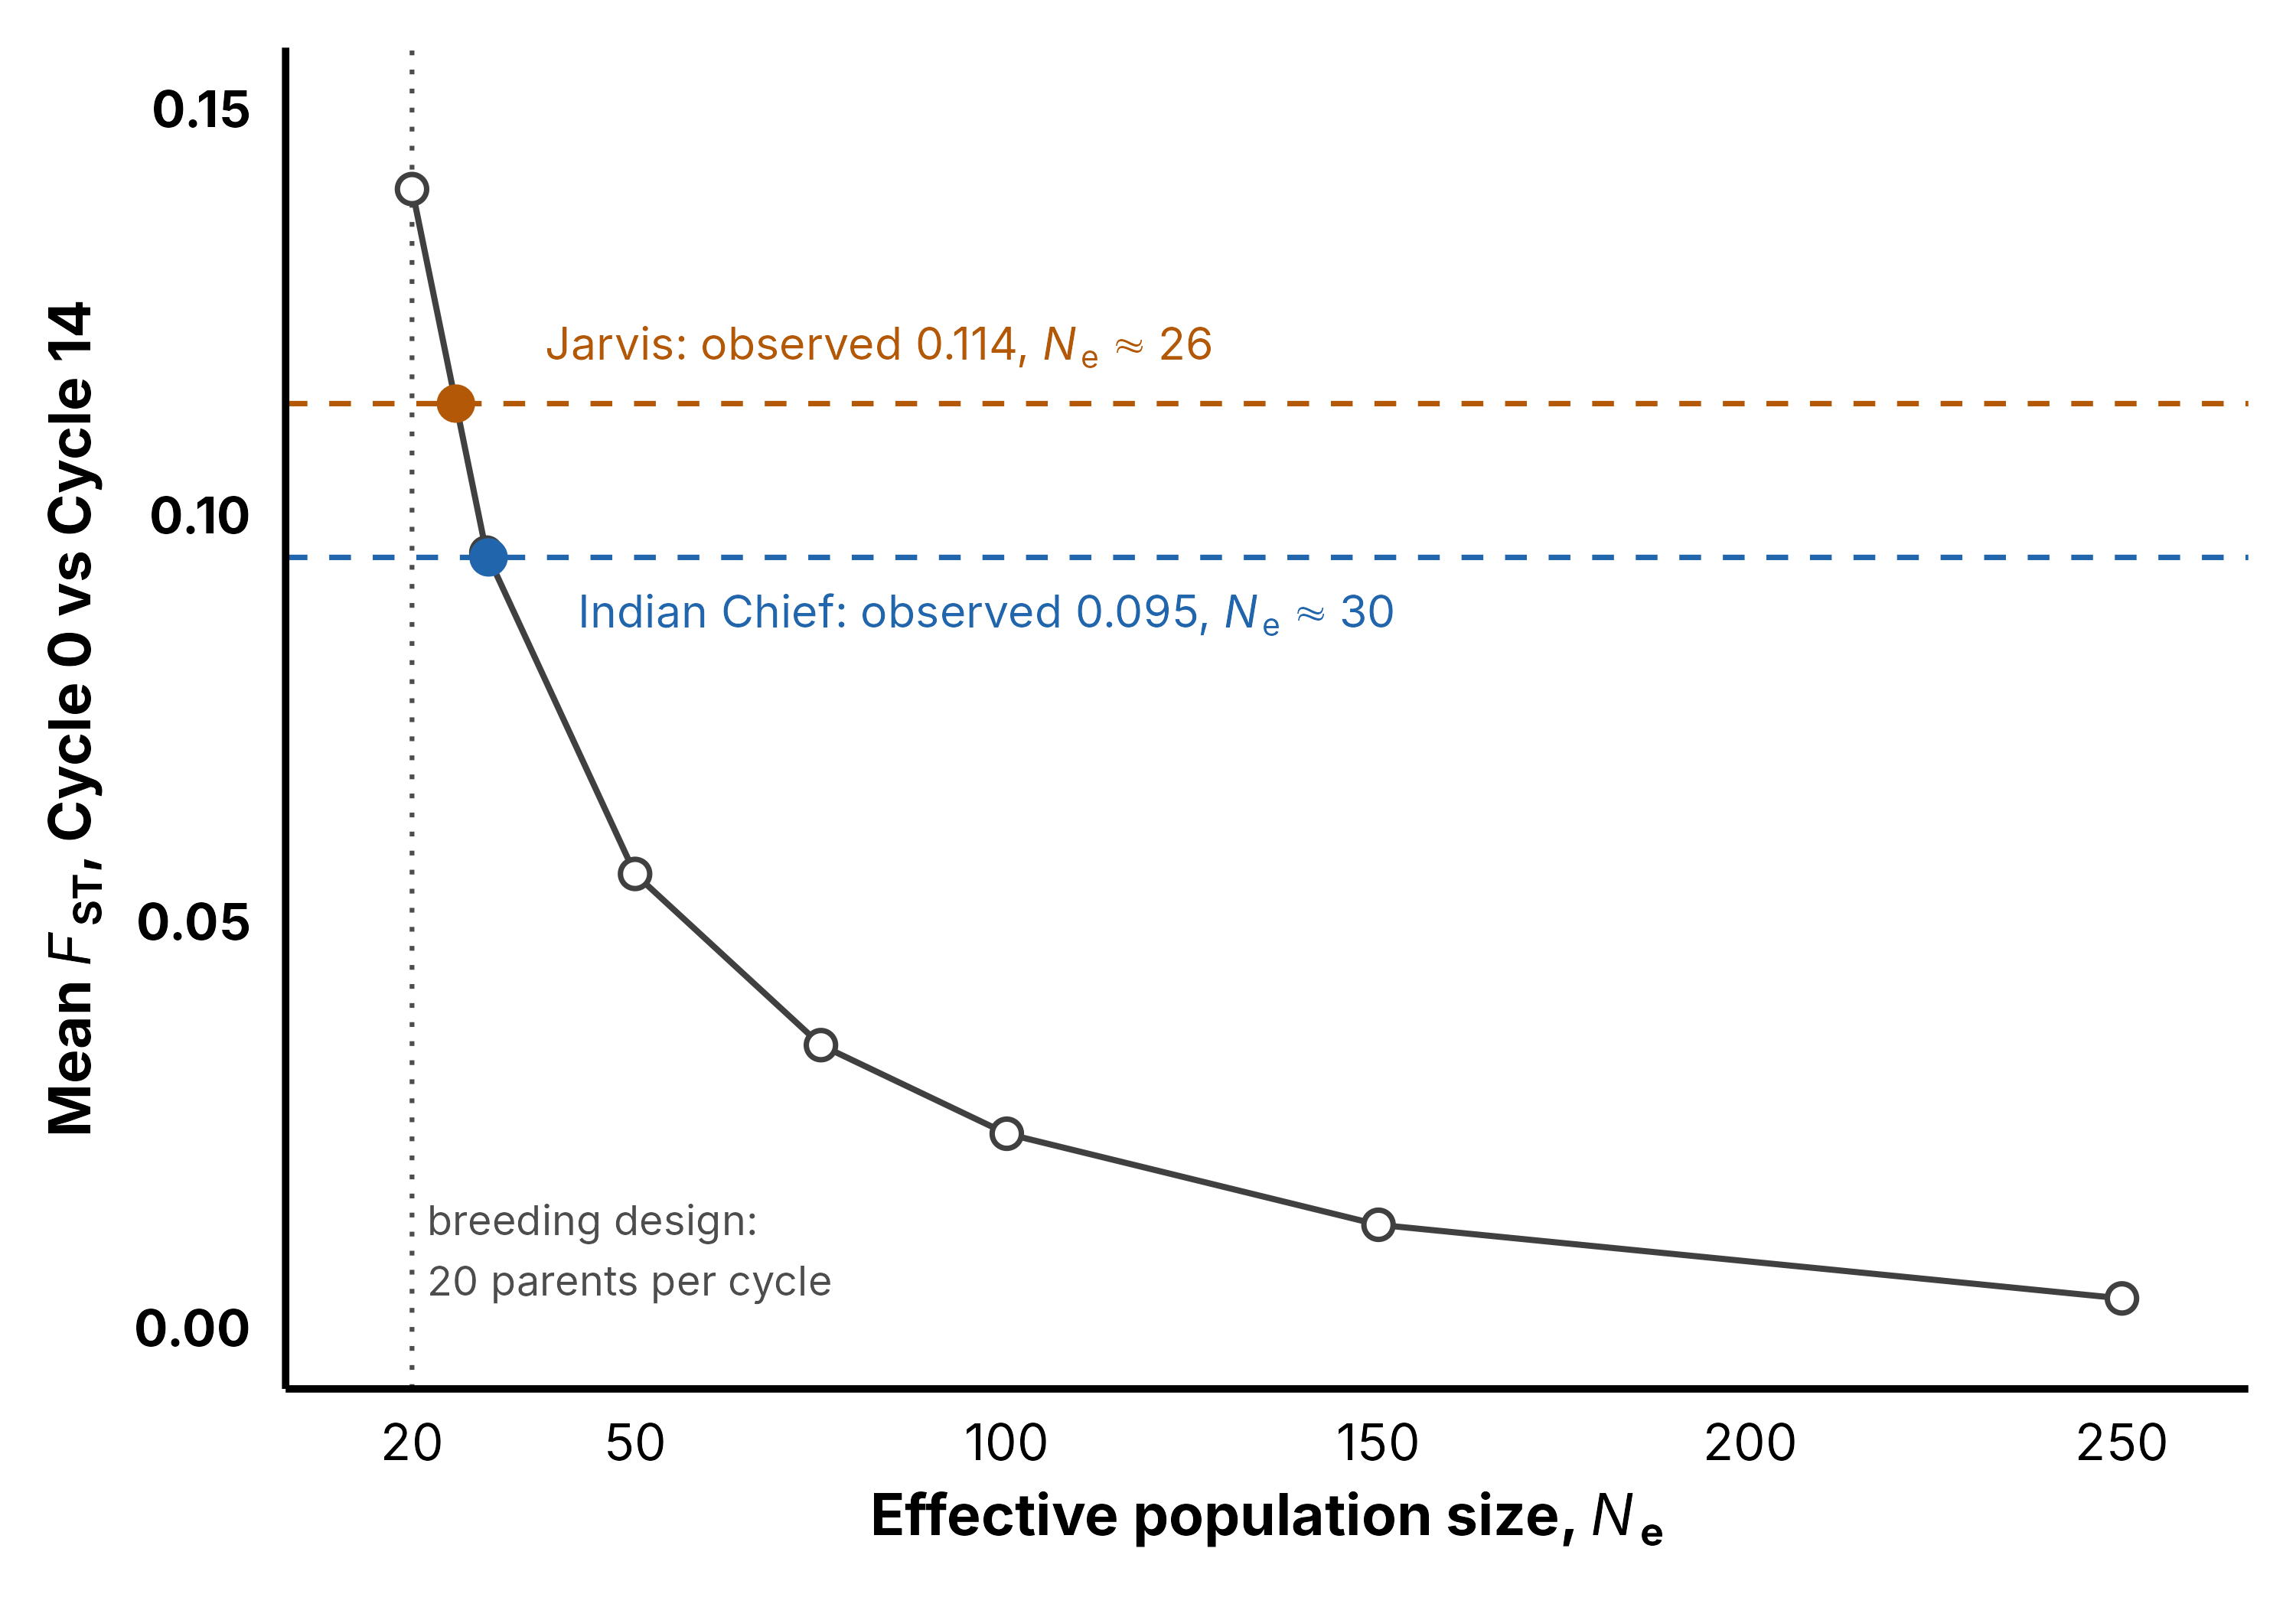
\includegraphics[width=0.75\textwidth]{figures/SuppFig_IC_J_Ne_drift.png}
\caption*{\textbf{Supplemental Figure S13.} \textbf{Effective population size of the Indian Chief and Jarvis recurrent-selection populations.} Genome-wide mean $F_{ST}$ between Cycle~0 and Cycle~14 expected under neutral Wright--Fisher drift for 14 generations across a range of effective population sizes ($N_e$; open circles), starting from the observed Cycle~0 allele frequencies and resampling the number of individuals sequenced at each site. Dashed lines give the observed values (Indian Chief 0.095, Jarvis 0.114), and filled circles mark the implied $N_e$, obtained by linear interpolation. The dotted line marks $N_e = 20$, the value expected when the 20 parents intermated in each cycle contribute equally.}
\end{figure}
\clearpage

\begin{figure}[p]
\centering
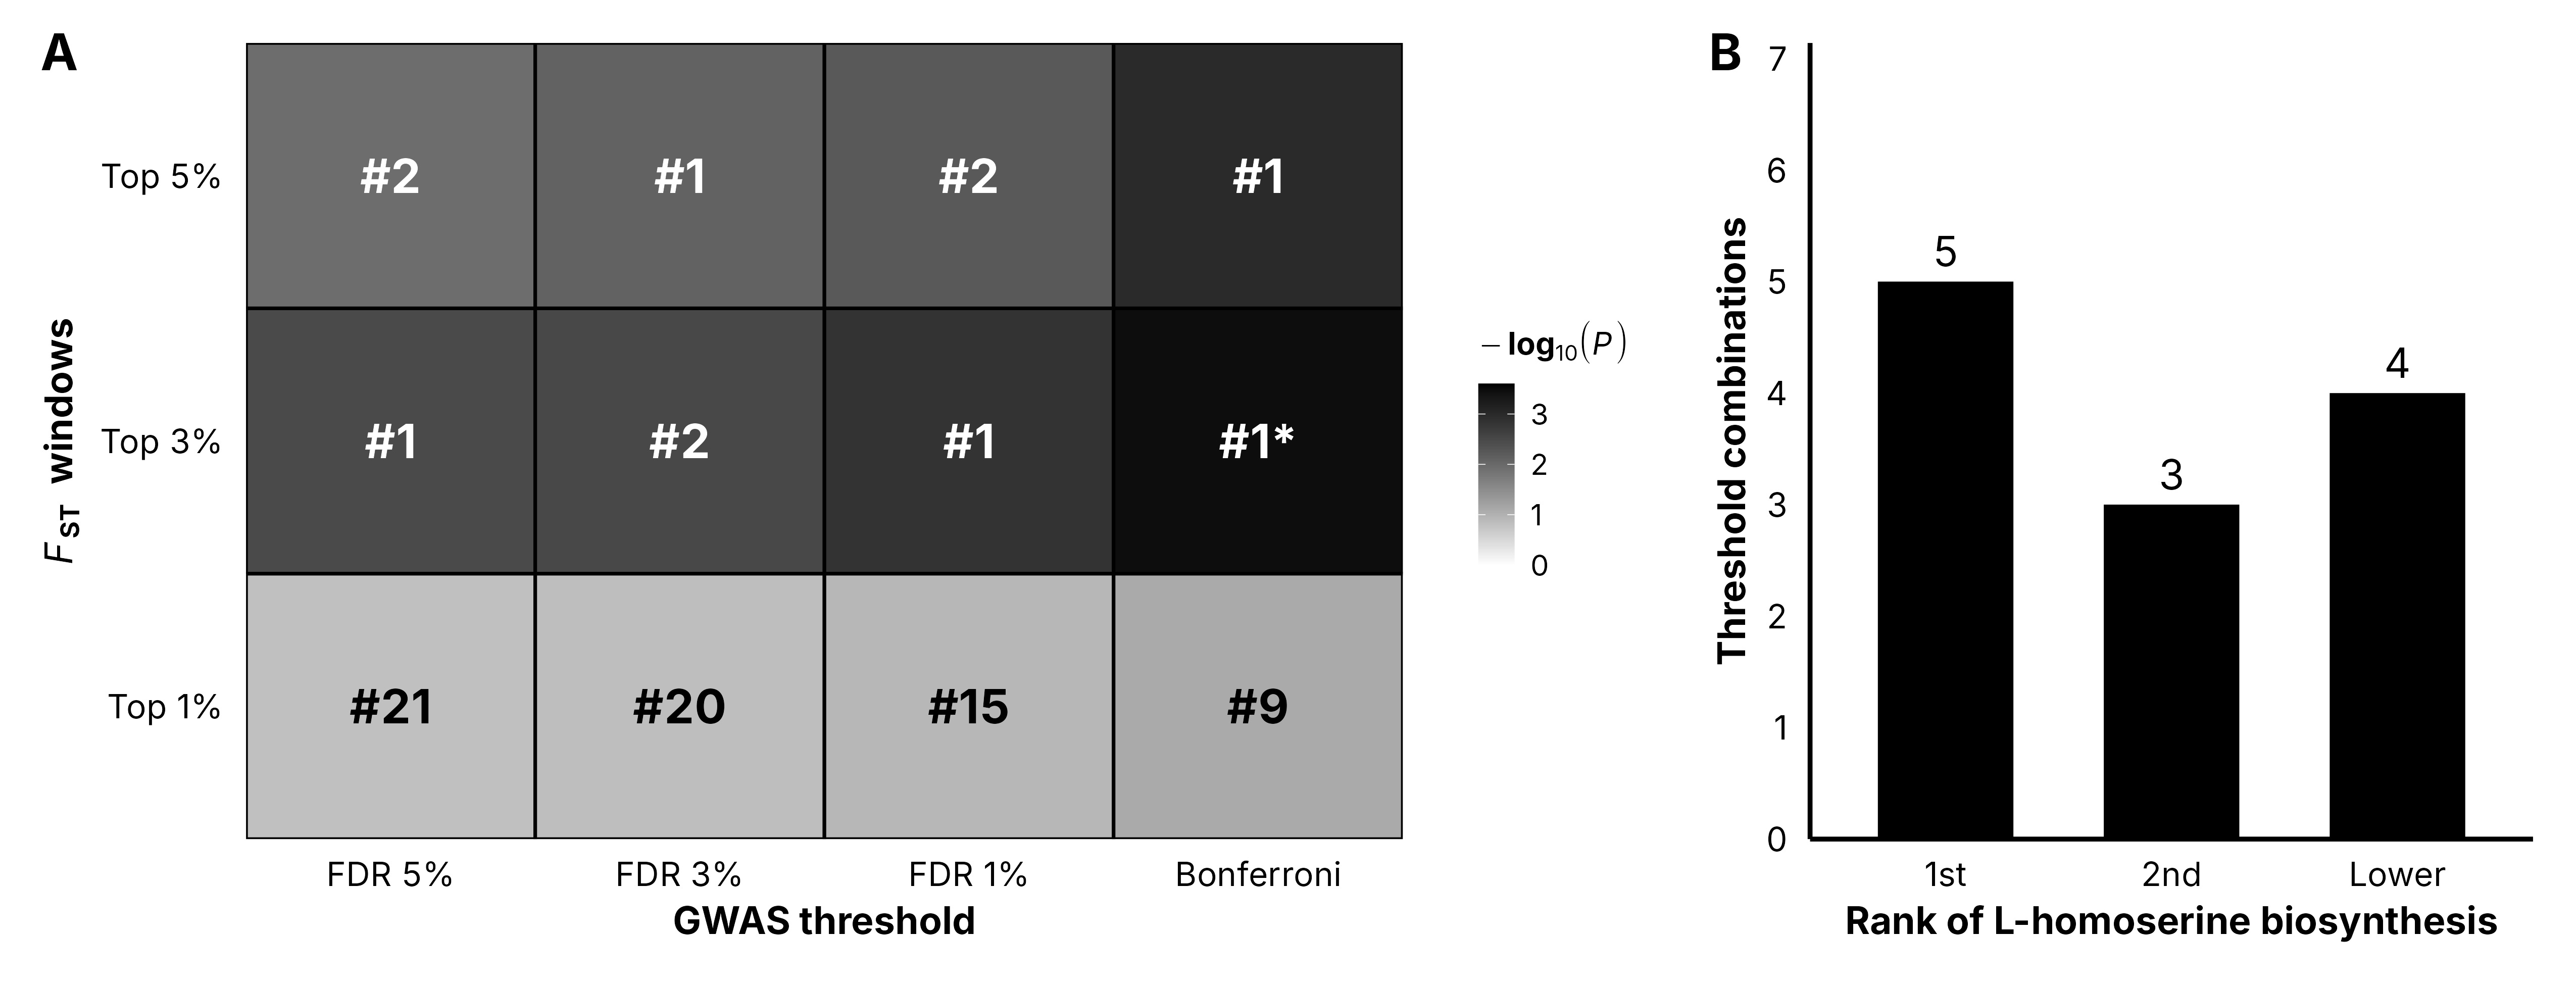
\includegraphics[width=0.75\textwidth]{figures/SuppFig_pathway_threshold_sensitivity.png}
\caption*{\textbf{Supplemental Figure S14.} \textbf{Sensitivity of the pathway recurrence test to candidate thresholds.} \textbf{(A)} L-homoserine biosynthesis across 12 combinations of GWAS threshold (columns, applied to both the amino acid and soil-N GWAS) and $F_{ST}$ window threshold (rows, Indian Chief and Jarvis). Shading gives $-\log_{10}$ of the pathway-specific permutation-based empirical $P$, labels give the rank of L-homoserine biosynthesis among the 468 CornCyc pathways, and an * marks $P < 0.05$ after correction across all pathways. At the top 1\%, the Indian Chief and Jarvis genes were no longer included and the pathway was hit by two analyses. \textbf{(B)} Number of the 12 combinations in which L-homoserine biosynthesis ranked first, second, or lower. Permutations, 20,000 per combination and 200,000 for the Bonferroni sets with the top 5\% and 3\% of windows.}
\end{figure}
\clearpage

\section*{Supplemental Tables}
Supplemental Tables S1--S22 are provided as separate CSV files.

\noindent\textbf{Supplemental Table S1.} \textbf{Free amino acid phenotypes across the Goodman--Buckler Association Panel.} Genotype-level values of the 78 amino acid phenotypes used for GWAS for 280 of the 282 lines (two years $\times$ two blocks, Columbia, Missouri): 20 absolute FAA concentrations, six biosynthetic-family composites, 20 ratios to the total free pool, 25 ratios to the family composite, four ratios between amino acids (N.D, N.E, N.Q, Q.E) and three whole-pool traits. Trait codes are defined in Supplemental Table~S2.

\noindent\textbf{Supplemental Table S2.} \textbf{Amino acid trait definitions.} Code and description of each of the 78 amino acid phenotypes in Supplemental Table~S1.

\noindent\textbf{Supplemental Table S3.} \textbf{Abundance, variability, and heritability of the 20 free amino acids.} For each FAA across 280 lines (278 for Tyr): median, mean, standard deviation, minimum, maximum, fold range, coefficient of variation, line mean broad-sense heritability ($H^2$), genomic heritability ($h^2$), and the Spearman correlation between 2017 and 2018 line means for the lines grown in both years.

\noindent\textbf{Supplemental Table S4.} \textbf{Heritability of free and protein-bound amino acid traits.} Line-mean and Cullis broad-sense heritability ($H^2$) and genomic heritability ($h^2$, with 95\% interval and permuted-phenotype null) for 40 FAA and 76 PBAA traits, with sample sizes and the Spearman correlation between 2017 and 2018 line means.

\noindent\textbf{Supplemental Table S5.} \textbf{Free vs.\ protein-bound amino acid pools.} Paired comparison of FAA and PBAA pools across matched lines for the total amino acid pool, the amino acid-derived N proxy, the proline fraction and the Asx + Glx + basic fraction (matched denominators): mean, median, standard deviation and coefficient of variation of each pool, fold difference and paired Wilcoxon $P$.

\noindent\textbf{Supplemental Table S6.} \textbf{Amino acid GWAS candidate genes.} All phenotype $\times$ SNP $\times$ gene combinations for SNPs significant at 5\% Benjamini--Hochberg FDR (per phenotype and model; MLM, BLINK, FarmCPU) within 25~kb of a B73 reference genome version 5 gene: 1,811 SNPs, 71 phenotypes, 3,693 genes. Includes significant models, lowest $P$ and FDR, whether the SNP is significant in $\geq$2 models, gene coordinates and distance. Positions are given on AGPv4 (\texttt{Pos\_v4}, the coordinate of the genotype data) and B73 reference genome version 5 (\texttt{Pos\_v5}, lifted with the chain file; \texttt{lift} = \texttt{gap} marks SNPs placed at the nearest aligned base); marker names carry the older AGPv3 coordinate.

\noindent\textbf{Supplemental Table S7.} \textbf{Amino acid GWAS loci.} The 2,152 loci were formed by merging FDR-significant SNP within 25 kb across phenotypes, with B73 reference genome version 5 coordinates, numbers of SNPs and phenotypes, best $P$, lead SNP (AGPv4 and v5 positions), supporting models, genes within 25 kb (or the nearest gene and its distance when none), top gene and its PANTHER family and GO terms.

\noindent\textbf{Supplemental Table S8.} \textbf{Genes in the chromosome~3 Asp/Pro QTL interval of the B64 $\times$ CML14 population.} The 1,578 B73 reference genome version 5 genes (1,386 protein-coding and 192 non-coding) within the 1.5-LOD support intervals (chr3:14.37--143.31~Mb) of the shared free Asp and Pro QTL (peak at 35.99~Mb), with gene coordinates, biotype, membership in the Asp and Pro intervals, distance to the QTL peak, gene name, PANTHER family, protein class, GO terms, kernel expression from qTeller \citep{qteller}, and overlap with candidates from the amino acid GWAS, soil N GWAS, and Indian Chief and Jarvis $F_{ST}$ scans.

\noindent\textbf{Supplemental Table S9.} \textbf{Soil N GWAS candidate genes.} The 448 B73 reference genome version 5 genes within 25~kb of the 216 soil-N SNPs (0--5~cm, 5\% FDR) that lie near a gene, one row per gene $\times$ SNP, with SNP statistics, overlap with other environmental GWAS, gene coordinates, distance, name, PANTHER family, protein class and GO terms.

\noindent\textbf{Supplemental Table S10.} \textbf{Environmental GWAS overlap test.} Observed vs.\ expected numbers of shared FDR-significant SNPs (MLM, BLINK and FarmCPU combined) for each site variable against the union of geographic variables (latitude, longitude, elevation; the variable itself excluded), and for soil N (0--5~cm) against each other variable. Expected $= n_1 n_2 / M$ with $M = 495{,}755$; one-sided hypergeometric $P$.

\noindent\textbf{Supplemental Table S11.} \textbf{Soil-N GWAS SNPs and their overlap with other environmental GWAS.} All 234 SNPs significant for soil N (0--5~cm) at 5\% FDR in MLM, BLINK or FarmCPU, with $P$ per model, MAF, number of models, whether each SNP is also FDR-significant in the GWAS of CEC, aridity, elevation, latitude, longitude, soil pH and soil N at 5--15~cm, and genes within 25~kb with the nearest gene's annotation.

\noindent\textbf{Supplemental Table S12.} \textbf{Genotype--environment correlation test for soil-N SNPs.} For each of the 234 soil-N SNPs, the Pearson correlation between genotype and soil N (0--5 and 5--15~cm), latitude, longitude, elevation, soil pH, CEC and aridity across 3,107 accessions; the SNP's genome-wide rank for each variable (\% of 495,755 SNPs with a stronger correlation); the most strongly correlated non-N variable; and the call: linked to environment (top 1\% for any non-N variable), not linked, or inconclusive (weak soil-N correlation, outside the top 5\%).

\noindent\textbf{Supplemental Table S13.} \textbf{Expectation test for the genotype–environment correlation.} Share of SNPs in the top 1\% of the genome for at least one geographic variable (latitude, longitude, elevation) or at least one of six non-N variables (adding soil pH, CEC, and aridity), for the whole genome, for SNPs in the top 1\% for correlation with soil N, for all soil N GWAS SNPs, and for those significant in $\geq$2 models, with binomial tests against the whole genome and against the soil N-correlated SNPs.

\noindent\textbf{Supplemental Table S14.} \textbf{Free amino acid metrics in Indian Chief and Jarvis, Cycle~0 vs. Cycle~14.} Eight pre-specified FAA metrics (total FAA per mg sample; Pro, Asn, Asp, Gln, and Gly fractions of total FAA; Asn + Gln + Arg + Lys + His per mg; FAA-derived N per mg) per population: biological-sample sizes, means, and medians per cycle, two-sided Wilcoxon rank-sum $P$, Benjamini--Hochberg-adjusted $P$ across the eight metrics, Cliff's $\delta$ (C14 vs. C0) and direction of change.

\noindent\textbf{Supplemental Table S15.} \textbf{Amino acid composition in Indian Chief and Jarvis, Cycle~0 vs.\ Cycle~14.} For each of the 20 free and 16 protein-bound amino acids, its fraction of the total pool per population and cycle: sample sizes, means, medians, Wilcoxon rank-sum $P$, Benjamini--Hochberg-adjusted $P$ across the amino acids of that pool, Cliff's $\delta$ and direction of change.

\noindent\textbf{Supplemental Table S16.} \textbf{Protein-bound amino acid metrics in Indian Chief and Jarvis, Cycle~0 vs.\ Cycle~14.} Six PBAA metrics (total PBAA per mg sample; proline, Asx and Glx fractions; Asx + Glx + Arg + Lys + His per mg; estimated PBAA-derived N per mg, with Asx and Glx at 1.5 N), with the same statistics as Supplemental Table~S14 and Benjamini--Hochberg adjustment across the six.

\noindent\textbf{Supplemental Table S17.} \textbf{Amino acid-derived N per mg sample in Indian Chief and Jarvis.} FAA-derived N, estimated PBAA-derived N, and estimated total amino acid-derived N per mg sample, per population and cycle, with Wilcoxon rank-sum $P$ and Benjamini--Hochberg-adjusted $P$ across the three measures.

\noindent\textbf{Supplemental Table S18.} \textbf{Indian Chief $F_{ST}$ windows, Cycle~0 vs. Cycle~14.} All 2,162 GenWin spline windows with chromosome, window number, start and end (B73 reference genome version 5), number of sites, mean per-site $F_{ST}$, whether the window is in the top 5\% ($F_{ST} \geq 0.157$), and the number and IDs of overlapping genes.

\noindent\textbf{Supplemental Table S19.} \textbf{Jarvis $F_{ST}$ windows, Cycle~0 vs.\ Cycle~14.} All 2,151 GenWin spline windows, with the same columns as Supplemental Table~S18 (top 5\%: $F_{ST} \geq 0.178$).

\noindent\textbf{Supplemental Table S20.} \textbf{Indian Chief candidate genes in top-5\% $F_{ST}$ windows.} The 2,001 genes overlapping the 109 top-5\% windows, with gene name, window coordinates and $F_{ST}$, whether the gene also lies in a top-5\% Jarvis window (\texttt{shared\_with\_other\_population}), PANTHER family and protein class, and Gene Ontology molecular function, biological process, and cellular component terms. Genes in the same window share one $F_{ST}$ value and are not independent.

\noindent\textbf{Supplemental Table S21.} \textbf{Jarvis candidate genes in top-5\% $F_{ST}$ windows.} The 1,179 genes overlap 106 of the 108 top-5\% windows (the other two contain no genes), with the same columns as Supplemental Table~S20.

\noindent\textbf{Supplemental Table S22.} \textbf{Expression responses of candidate genes to N supply in public maize RNA-seq.} Reanalysis of published maize RNA-seq studies of root, leaf, shoot, and whole-seedling tissue (no kernel data) for the candidate genes named in the text and \textit{ASN3}.


\bibliographystyle{oup-abbrvnat}
\bibliography{sn-bibliography}
\end{document}
